% Options for packages loaded elsewhere
\PassOptionsToPackage{unicode}{hyperref}
\PassOptionsToPackage{hyphens}{url}
\PassOptionsToPackage{dvipsnames,svgnames,x11names}{xcolor}
\documentclass[
  11pt,
]{article}
\usepackage{xcolor}
\usepackage[margin=1in]{geometry}
\usepackage{amsmath,amssymb}
\setcounter{secnumdepth}{-\maxdimen} % remove section numbering
\usepackage{iftex}
\ifPDFTeX
  \usepackage[T1]{fontenc}
  \usepackage[utf8]{inputenc}
  \usepackage{textcomp} % provide euro and other symbols
\else % if luatex or xetex
  \usepackage{unicode-math} % this also loads fontspec
  \defaultfontfeatures{Scale=MatchLowercase}
  \defaultfontfeatures[\rmfamily]{Ligatures=TeX,Scale=1}
\fi
\usepackage{lmodern}
\ifPDFTeX\else
  % xetex/luatex font selection
\fi
% Use upquote if available, for straight quotes in verbatim environments
\IfFileExists{upquote.sty}{\usepackage{upquote}}{}
\IfFileExists{microtype.sty}{% use microtype if available
  \usepackage[]{microtype}
  \UseMicrotypeSet[protrusion]{basicmath} % disable protrusion for tt fonts
}{}
\makeatletter
\@ifundefined{KOMAClassName}{% if non-KOMA class
  \IfFileExists{parskip.sty}{%
    \usepackage{parskip}
  }{% else
    \setlength{\parindent}{0pt}
    \setlength{\parskip}{6pt plus 2pt minus 1pt}}
}{% if KOMA class
  \KOMAoptions{parskip=half}}
\makeatother
\usepackage{longtable,booktabs,array}
\usepackage{caption}
\captionsetup[table]{skip=6pt}
\newcounter{none} % for unnumbered tables
\usepackage{calc} % for calculating minipage widths
% Correct order of tables after \paragraph or \subparagraph
\usepackage{etoolbox}
\makeatletter
\patchcmd\longtable{\par}{\if@noskipsec\mbox{}\fi\par}{}{}
\makeatother
% Allow footnotes in longtable head/foot
\IfFileExists{footnotehyper.sty}{\usepackage{footnotehyper}}{\usepackage{footnote}}
\makesavenoteenv{longtable}
\usepackage{graphicx}
\makeatletter
\newsavebox\pandoc@box
\newcommand*\pandocbounded[1]{% scales image to fit in text height/width
  \sbox\pandoc@box{#1}%
  \Gscale@div\@tempa{\textheight}{\dimexpr\ht\pandoc@box+\dp\pandoc@box\relax}%
  \Gscale@div\@tempb{\linewidth}{\wd\pandoc@box}%
  \ifdim\@tempb\p@<\@tempa\p@\let\@tempa\@tempb\fi% select the smaller of both
  \ifdim\@tempa\p@<\p@\scalebox{\@tempa}{\usebox\pandoc@box}%
  \else\usebox{\pandoc@box}%
  \fi%
}
% Set default figure placement to htbp
\def\fps@figure{htbp}
\makeatother
\setlength{\emergencystretch}{3em} % prevent overfull lines
\providecommand{\tightlist}{%
  \setlength{\itemsep}{0pt}\setlength{\parskip}{0pt}}
\usepackage{bookmark}
\IfFileExists{xurl.sty}{\usepackage{xurl}}{} % add URL line breaks if available
\urlstyle{same}
% fallback for those not using the hyperref driver hyperxmp:
\makeatletter
\@ifundefined{xmpquote}{\newcommand{\xmpquote}[1]{#1}}{}
\makeatother
\hypersetup{
  pdftitle={QuantBloom Terminal},
  pdfauthor={QuantBloom Research},
  colorlinks=true,
  linkcolor={RoyalBlue},
  filecolor={Maroon},
  citecolor={Blue},
  urlcolor={RoyalBlue},
  pdfcreator={LaTeX via pandoc}}

\title{QuantBloom Terminal}
\usepackage{etoolbox}
\makeatletter
\providecommand{\subtitle}[1]{% add subtitle to \maketitle
  \apptocmd{\@title}{\par {\large #1 \par}}{}{}
}
\makeatother
\subtitle{A Technical Whitepaper --- Machine Learning, Trading
Strategies, and the Mathematics Behind Them}
\author{QuantBloom Research}
\date{Version 1.0}

\begin{document}
\maketitle

{
\setcounter{tocdepth}{2}
\tableofcontents
}
\subsection{Abstract}\label{abstract}

QuantBloom Terminal is a single-page, browser-native quantitative
research and trading environment modelled on the workflow of a
professional trading desk. It unifies market data, advanced charting, a
machine-learning signal pipeline, an honest backtesting engine, a
risk-gated paper-trading bot, a broad suite of portfolio and derivatives
analytics, and a power/commodities pricing desk into a single 37-panel
terminal. The system is written in JavaScript end to end --- a
React/Vite front end and an Express API --- with every numerically
load-bearing computation implemented as a pure, unit-tested module (332
tests at the time of writing).

This paper documents the system in depth. Its emphasis is on the
\textbf{mathematics} of the trading and machine-learning components: the
feature construction and triple-barrier labelling; the three in-app
model families (regularised logistic regression, gradient-boosted
decision trees, and a PCA latent-factor model built on a from-scratch
Jacobi eigensolver) and their ensemble; the metrics used to judge them;
and --- most importantly --- the \textbf{overfitting guards}
(Probabilistic and Deflated Sharpe ratios, and the Probability of
Backtest Overfitting via combinatorially-symmetric cross-validation)
that form the publish gate. We also document the point-in-time
backtester, the rule-based strategies, the trading bot's risk gate and
bracket/trailing-stop machinery, the portfolio analytics (mean-variance
optimisation, three-method Value-at-Risk, factor regression, DCF, and
time-value-of-money), and the power-markets desk (merit-order dispatch,
locational marginal pricing under transmission congestion, spark
spreads, and a Monte-Carlo heat-rate call option) derived from a Citadel
power \& gas primer.

A recurring theme is \textbf{intellectual honesty}. The system is
explicit about the difference between \emph{observed} and
\emph{modelled} quantities, and its most important design decision ---
the publish gate --- is built to reject models that do not demonstrably
beat a buy-and-hold benchmark out of sample. As documented in Section
16, none of the daily-bar models currently clear that bar. We treat that
as the tooling working correctly, not as a failure to be tuned away.

\begin{center}\rule{0.5\linewidth}{0.5pt}\end{center}

\subsection{1. Introduction and
Motivation}\label{introduction-and-motivation}

Professional trading terminals --- the Bloomberg Terminal being the
archetype --- succeed because they collapse the distance between a
question and its answer. A trader types a ticker and a mnemonic and is
instantly looking at the relevant chart, fundamental, or analytic.
QuantBloom pursues the same ergonomic goal in a browser, but with a
second, equally important commitment: \textbf{every number it shows
should be traceable to a tested computation, and every modelled quantity
should be labelled as such.}

The terminal is organised as a dashboard of independent panels. Each
panel is a self-contained React component that polls the API for the
data it needs and renders a focused view --- a chart, a screener, a risk
report, a pricing calculator. A global command palette (\texttt{Ctrl+K},
the Bloomberg \texttt{TICKER\ \textless{}GO\textgreater{}} pattern) sets
the active symbol across the whole terminal or jumps to any panel; any
panel can be popped out into its own live browser window
(\texttt{Ctrl+Shift+M}) to spread work across monitors.

\begin{figure}
\centering
\pandocbounded{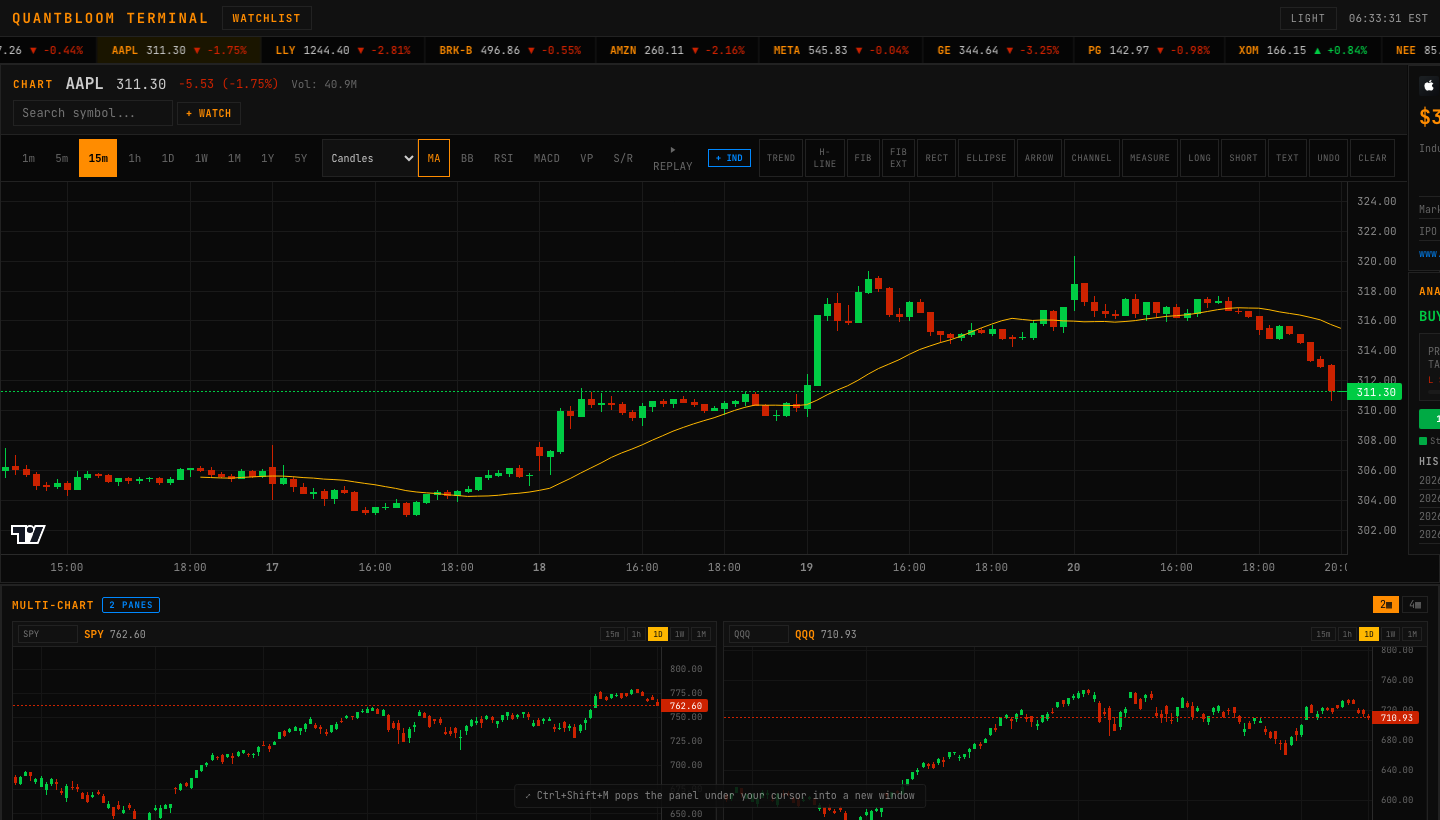
\includegraphics[keepaspectratio,alt={The QuantBloom hero view: navigation, the cross-asset ticker, and the primary chart with a moving-average overlay.}]{img/hero.png}}
\caption{The QuantBloom hero view: navigation, the cross-asset ticker,
and the primary chart with a moving-average overlay.}
\end{figure}

\emph{Figure 1. The terminal hero --- command bar, cross-asset ticker
tape, and the primary interactive chart.}

Beneath the UI sit three intellectual pillars, each of which this paper
treats in detail:

\begin{enumerate}
\def\labelenumi{\arabic{enumi}.}
\item
  \textbf{Signal research} --- a supervised-learning pipeline that turns
  OHLCV bars into point-in-time features, labels them with a
  triple-barrier scheme, trains several model families, and ---
  crucially --- refuses to ``publish'' a model that cannot beat
  buy-and-hold out of sample after correction for multiple testing.
\item
  \textbf{Execution} --- a paper-trading bot whose every order passes a
  hard-coded risk gate, can carry broker-side stop-loss/take-profit
  brackets and a live trailing stop, and can be driven either by
  transparent rule strategies or by a selected ML model.
\item
  \textbf{Analytics} --- a broad set of desk tools: mean-variance
  portfolio optimisation, three-method VaR, factor regression,
  discounted-cash-flow valuation, time-value-of-money, and a
  power-markets pricing desk.
\end{enumerate}

\subsubsection{1.1 Design principles}\label{design-principles}

\begin{itemize}
\tightlist
\item
  \textbf{Tested maths, not trusted maths.} Anything that produces a
  number a user might act on lives in a pure module with a dedicated
  test file that asserts its \emph{defining properties}, not merely that
  it runs.
\item
  \textbf{Point-in-time everywhere.} Both the live signal path and the
  backtester compute features from bars \texttt{{[}0..t{]}} only; a
  model never sees a bar it could not have seen in production.
  Train/live feature parity is enforced.
\item
  \textbf{Observed vs.~modelled.} Panels that display a model (DCF, VaR,
  the power desk, any ML signal) say so in the interface. The system
  never presents a simulation as an observation.
\item
  \textbf{Honest gating.} The publish gate is deliberately demanding.
  Most strategies fail it, which is the correct outcome for daily-bar
  technical analysis on liquid names.
\end{itemize}

\begin{center}\rule{0.5\linewidth}{0.5pt}\end{center}

\subsection{2. System Architecture}\label{system-architecture}

\subsubsection{2.1 Runtime shape}\label{runtime-shape}

QuantBloom is two processes:

\begin{itemize}
\tightlist
\item
  A \textbf{React 18 + Vite} front end (\texttt{src/}) that renders the
  terminal and holds all UI state through the React Context API and
  \texttt{useReducer}.
\item
  An \textbf{Express} API (\texttt{server.js}, \textasciitilde2,900
  lines) that proxies market data, computes the shared
  technical-indicator payload, and hosts the bot, backtest, and
  model-training routes (\textasciitilde50 routes in total).
\end{itemize}

For local or Docker deployment the Express server also serves the built
front-end, so \texttt{node\ server.js} is a single self-contained
process. On a serverless host (Vercel) the same \texttt{app} is exported
as a function; the stateful trading bot and file-based model persistence
degrade gracefully to in-memory there, and the UI documents that the bot
needs a persistent process.

\subsubsection{2.2 Module layout}\label{module-layout}

The numerically important code is deliberately isolated from the UI and
the server so it can be tested in a plain Node process:

{\def\LTcaptype{none} % do not increment counter
\begin{longtable}[]{@{}
  >{\raggedright\arraybackslash}p{(\linewidth - 4\tabcolsep) * \real{0.3333}}
  >{\raggedright\arraybackslash}p{(\linewidth - 4\tabcolsep) * \real{0.3333}}
  >{\raggedright\arraybackslash}p{(\linewidth - 4\tabcolsep) * \real{0.3333}}@{}}
\toprule\noalign{}
\begin{minipage}[b]{\linewidth}\raggedright
Concern
\end{minipage} & \begin{minipage}[b]{\linewidth}\raggedright
Module(s)
\end{minipage} & \begin{minipage}[b]{\linewidth}\raggedright
Tested in
\end{minipage} \\
\midrule\noalign{}
\endhead
\bottomrule\noalign{}
\endlastfoot
Options pricing \& Greeks & \texttt{blackscholes.js} &
\texttt{test/blackscholes.test.mjs} \\
OLS regression & \texttt{regression.js} &
\texttt{test/regression.test.mjs} \\
Mean-variance optimisation & \texttt{portfolio-math.js} &
\texttt{test/portfolio-math.test.mjs} \\
Feature engineering \& labels & \texttt{bot/features.js} &
\texttt{test/*} \\
Logistic / PCA / ensemble models & \texttt{bot/model.js} &
\texttt{test/model.test.mjs}, \texttt{test/ensemble.test.mjs} \\
Gradient-boosted trees & \texttt{bot/gbm.js} &
\texttt{test/gbm.test.mjs} \\
Eigendecomposition (Jacobi) & \texttt{bot/eigen.js} &
\texttt{test/eigen.test.mjs} \\
PCA & \texttt{bot/pca.js} & \texttt{test/pca.test.mjs} \\
Overfitting statistics & \texttt{bot/statistics.js} &
\texttt{test/statistics.test.mjs} \\
Backtester & \texttt{bot/backtest.js} &
\texttt{test/backtest.test.mjs} \\
Risk gate & \texttt{bot/risk-gate.js} &
\texttt{test/risk-gate.test.mjs} \\
Brackets / trailing stop & \texttt{bot/brackets.js} &
\texttt{test/brackets.test.mjs} \\
Strategies & \texttt{bot/strategies.js} &
\texttt{test/contrarian.test.mjs} \\
Chart-type transforms & \texttt{charting/chart-types.js} &
\texttt{test/chart-types.test.mjs} \\
Indicator series & \texttt{charting/indicators.js} &
\texttt{test/indicators-series.test.mjs} \\
Drawing maths & \texttt{charting/drawing-math.js} &
\texttt{test/drawing-math.test.mjs} \\
Volume profile \& structure & \texttt{charting/volume-profile.js} &
\texttt{test/volume-profile.test.mjs} \\
Bar-replay state & \texttt{charting/replay.js} &
\texttt{test/replay.test.mjs} \\
Formula interpreter & \texttt{charting/formula.js} &
\texttt{test/formula.test.mjs} \\
Power markets & \texttt{charting/power.js} &
\texttt{test/power.test.mjs} \\
Time value of money & \texttt{bot/tvm.js} &
\texttt{test/tvm.test.mjs} \\
Command-palette logic & \texttt{src/lib/command.js} &
\texttt{test/command.test.mjs} \\
\end{longtable}
}

The rule is uniform: a panel is a thin rendering layer over a tested
module.

\begin{center}\rule{0.5\linewidth}{0.5pt}\end{center}

\subsection{3. Market-Data Layer}\label{market-data-layer}

QuantBloom runs on free-tier and public data. Yahoo Finance (no key
required) provides OHLCV candles across timeframes and powers charts,
quotes, screeners, backtests, and the entire model lab. Optional keyed
providers enrich specific panels --- Finnhub (fundamentals, analyst
ratings, calendars), FRED (macro and the yield curve), Alpha Vantage
(quote fallback), Marketaux and NewsAPI (news with sentiment). A missing
key disables only the panel that needs it; the terminal runs with none
set.

The server maintains a small in-memory cache to smooth polling and
shares one canonical \textbf{technical-analysis payload builder}
(\texttt{bot/indicators.js}, \texttt{computeTechnical}) between the live
\texttt{/api/v1/technical} route and the backtester, so a rule strategy
sees byte-identical indicator inputs whether it is running live or being
backtested. This is a deliberate anti-divergence measure: the single
most common source of ``it worked in the backtest'' errors is a mismatch
between research and production feature code.

\begin{center}\rule{0.5\linewidth}{0.5pt}\end{center}

\subsection{4. The Charting Engine}\label{the-charting-engine}

The chart is built on \texttt{lightweight-charts} and extended with a
family of tested, clean-room implementations of standard chart
constructions and indicators.

\subsubsection{4.1 Chart types}\label{chart-types}

Eight chart types are available. Several are native series styles; three
are deterministic transforms of the candle series implemented in
\texttt{charting/chart-types.js}:

\textbf{Heikin-Ashi.} A smoothing transform that averages the OHLC to
damp noise:

\[
\begin{aligned}
\text{HA}_\text{close} &= \tfrac{1}{4}(O + H + L + C)\\
\text{HA}_\text{open}  &= \tfrac{1}{2}\big(\text{HA}_\text{open}^{\,t-1} + \text{HA}_\text{close}^{\,t-1}\big)\\
\text{HA}_\text{high}  &= \max(H,\ \text{HA}_\text{open},\ \text{HA}_\text{close})\\
\text{HA}_\text{low}   &= \min(L,\ \text{HA}_\text{open},\ \text{HA}_\text{close})
\end{aligned}
\]

with the seed \(\text{HA}_\text{open}^{\,0} = \tfrac{1}{2}(O_0 + C_0)\).
The transform preserves the time axis one-to-one; the test suite asserts
that the close equals the OHLC mean, the open is the average of the
previous HA open/close, and the high/low bound both the HA body and the
true range.

\textbf{Renko} rebuilds the series as fixed-size ``bricks'': a new brick
of height equal to the box size (defaulting to the average true range)
is emitted only when price moves a full box beyond the last brick's
close, discarding sub-box noise. Because Renko and Line-Break have no
uniform time axis, bricks are emitted with strictly increasing synthetic
times so a candlestick renderer can display them.

\textbf{N-line break} (default \(N=3\)) draws a new line only when the
close breaks beyond the extreme of the last \(N\) lines; smaller moves
are absorbed, so a reversal requires conviction.

\subsubsection{4.2 Indicator series
library}\label{indicator-series-library}

\texttt{charting/indicators.js} computes full \textbf{series} (not the
point-in-time snapshots the bot uses) for plotting. It provides SMA,
EMA, WMA, anchored VWAP, Bollinger, Keltner, Donchian, Parabolic SAR and
SuperTrend as price overlays, and RSI, MACD, Stochastic, CCI, Williams
\%R, ATR and OBV as sub-pane oscillators. A registry carries each
indicator's pane, colour, and parameters so the overlay manager is
data-driven. Representative definitions:

\[
\text{EMA}_t = \alpha\,P_t + (1-\alpha)\,\text{EMA}_{t-1},\quad \alpha = \frac{2}{n+1}
\]

\[
\text{RSI}_t = 100 - \frac{100}{1 + \text{RS}_t},\qquad
\text{RS}_t = \frac{\overline{\text{gain}}_n}{\overline{\text{loss}}_n}
\]

with Wilder's smoothing of the average gain and loss. The test suite
asserts the defining behaviours --- RSI is 100 on a monotonic rise and
\textasciitilde0 on a decline and stays in \([0,100]\); the MACD
histogram equals MACD minus signal; Bollinger bands straddle the middle
band and widen with volatility; Donchian's upper/lower equal the rolling
max-high/min-low; OBV rises on up-closes and falls on down-closes.

\subsubsection{4.3 Volume profile and market
structure}\label{volume-profile-and-market-structure}

\texttt{charting/volume-profile.js} buckets traded volume by
\textbf{price} rather than time, distributing each bar's volume across
the price buckets its high-low range spans weighted by overlap. It
returns the \textbf{point of control} (the busiest price), and a
\textbf{value area} computed by expanding outward from the POC --- at
each step taking whichever adjacent bucket holds more volume --- until
70\% of total volume is enclosed. A companion \texttt{supportResistance}
clusters swing pivots (bars that are the strict extreme within a
\(\pm k\) window) into strength-ranked levels. The overlay renders as a
right-edge histogram with the POC and value area highlighted, plus
dashed support/resistance lines.

\subsubsection{4.4 Drawing tools, replay, and
multi-chart}\label{drawing-tools-replay-and-multi-chart}

The drawing layer stores anchors as \texttt{\{time,\ price\}} (so they
stay pinned through pan/zoom) and offers trend lines, horizontal lines,
Fibonacci retracement and extension, channels, ellipses, arrows, a
\textbf{measure} tool (Δprice, Δ\%, bars), and a \textbf{long/short
position} tool with a live reward-to-risk readout. The numeric parts are
factored into \texttt{charting/drawing-math.js} and tested --- e.g.,
\texttt{positionRR(100,\ 110,\ 95)} returns a long trade with R:R 2.

\textbf{Bar replay} (\texttt{charting/replay.js}) reveals history one
bar at a time from a cursor so a setup can be reviewed exactly as it
looked then; every layer --- base series, indicators, drawings, volume
profile --- slices to the same cursor, so nothing leaks the future. The
key test asserts \texttt{sliceUpTo} never returns a bar whose time
exceeds the cursor.

A \textbf{multi-chart} panel renders a 2- or 4-pane grid of fully
independent charts, each with its own symbol, timeframe, and data feed.

\begin{figure}
\centering
\pandocbounded{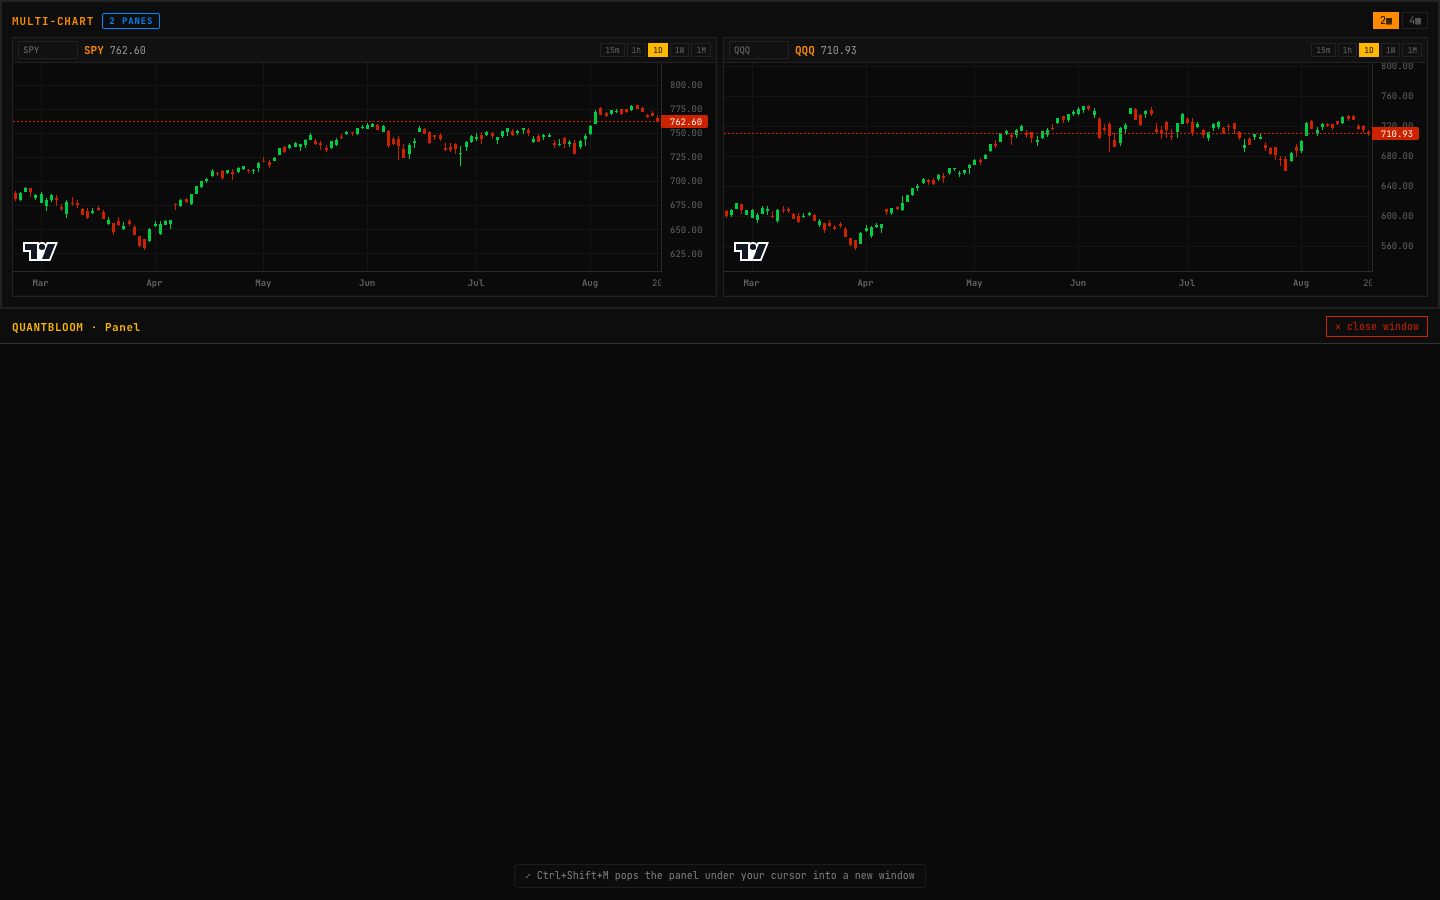
\includegraphics[keepaspectratio,alt={Independent multi-chart grid, each pane with its own symbol and timeframe.}]{img/multi-chart.png}}
\caption{Independent multi-chart grid, each pane with its own symbol and
timeframe.}
\end{figure}

\emph{Figure 2. The multi-chart grid --- four independent, live charts.}

\subsubsection{4.5 A neutral custom-indicator
language}\label{a-neutral-custom-indicator-language}

\texttt{charting/formula.js} is a small, sandboxed expression
interpreter --- a tokeniser, a recursive-descent parser, and an AST
evaluator over a fixed whitelist of series
(\texttt{open,\ high,\ low,\ close,\ volume,\ hl2,\ hlc3,\ ohlc4}),
functions (\texttt{sma,\ ema,\ stdev,\ rsi,\ abs,\ max,\ min}), and
operators. It is \textbf{not} \texttt{eval}: there is no grammar rule
that can produce a JavaScript global, prototype, or arbitrary call, so a
user formula cannot reach outside itself. The test suite includes an
explicit sandbox battery --- \texttt{constructor}, \texttt{window},
\texttt{eval}, \texttt{\_\_proto\_\_} and member access are all rejected
--- alongside correctness tests (SMA equals the hand-average,
\texttt{close\ -\ sma(close,20)} is an oscillator).

\begin{figure}
\centering
\pandocbounded{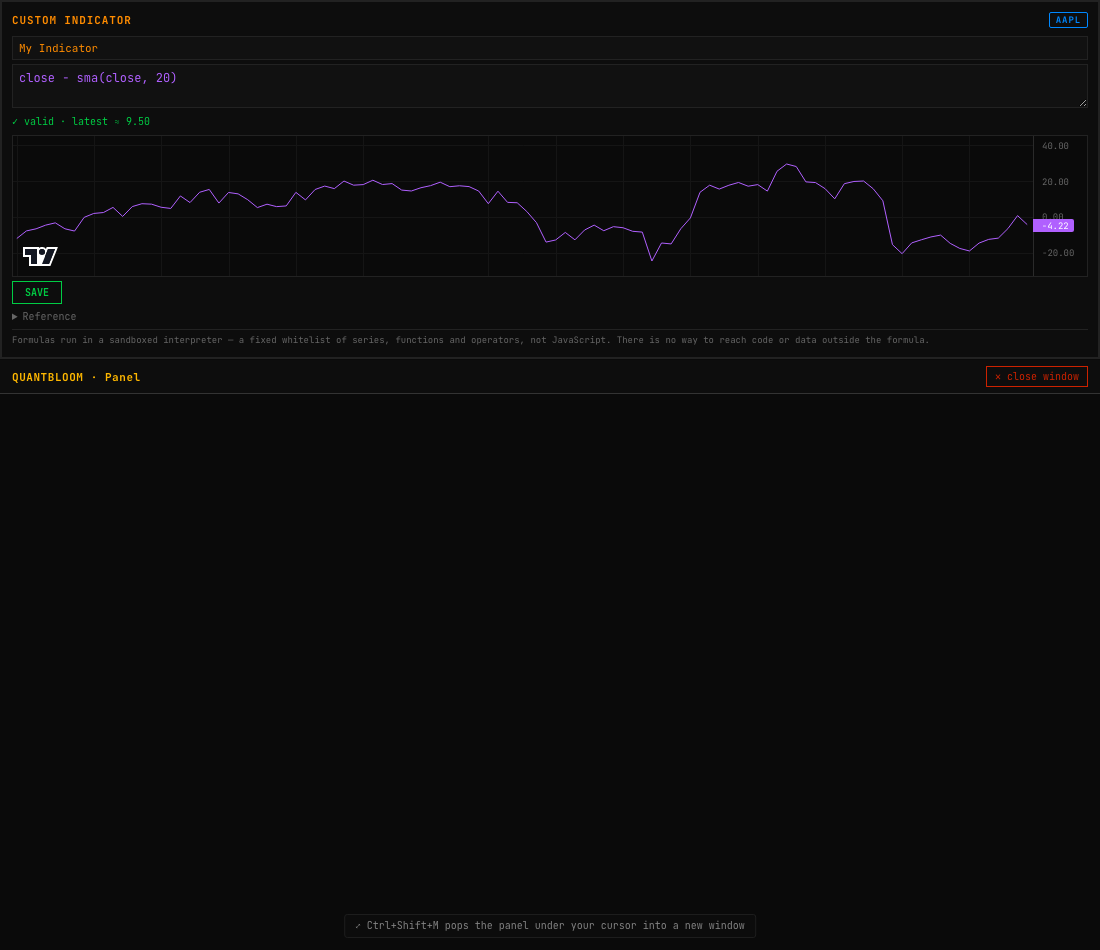
\includegraphics[keepaspectratio,alt={The custom-indicator editor with live validation and a preview chart.}]{img/custom-indicator.png}}
\caption{The custom-indicator editor with live validation and a preview
chart.}
\end{figure}

\emph{Figure 3. The sandboxed custom-indicator editor: a formula, live
validation, and a preview of the resulting series.}

\begin{center}\rule{0.5\linewidth}{0.5pt}\end{center}

\subsection{5. Feature Engineering and
Labelling}\label{feature-engineering-and-labelling}

The ML pipeline begins by turning a candle series into a supervised
dataset. This is the most consequential and error-prone part of any
trading-ML system, and the one where point-in-time discipline matters
most.

\subsubsection{5.1 Point-in-time features}\label{point-in-time-features}

\texttt{bot/features.js} computes, at each bar \(t\), a
\textbf{19-dimensional} feature vector from bars \([0..t]\) only. The
features are chosen to be scale-free and to span several economic ideas
--- momentum, mean-reversion, trend regime, range position, and
volatility regime:

\begin{itemize}
\tightlist
\item
  Returns: \texttt{ret1}, \texttt{ret5}, \texttt{roc20} (rate of
  change).
\item
  Trend/location: \texttt{priceVsSma50}, \texttt{priceVsSma200},
  \texttt{sma20Slope}.
\item
  Oscillators: \texttt{rsi14}, \texttt{rsiSlope}, \texttt{macdHist},
  \texttt{stoch}.
\item
  Bands/range: \texttt{bollingerPct}, \texttt{distFrom120High},
  \texttt{distFrom120Low}.
\item
  Volume/vol: \texttt{volumeRatio}, \texttt{volatility},
  \texttt{volRegime}, \texttt{atrPct}.
\end{itemize}

Every value passes through a finite-guard so no
\texttt{NaN}/\texttt{Infinity} can reach a model. The dataset builder
uses a \textbf{200-bar warm-up} so that long-lookback features (SMA-200)
are fully formed from the first training row.

\subsubsection{5.2 Cross-asset (market-relative)
features}\label{cross-asset-market-relative-features}

Optionally, five \textbf{market-relative} features are appended,
computed against a benchmark (SPY) whose closes are aligned to the
stock's bar times with carry-forward across gaps:

\[
\text{excessRet}_k = \frac{P_t}{P_{t-k}} - 1 - \left(\frac{B_t}{B_{t-k}} - 1\right),\quad k \in \{1,5\}
\]

plus a 20-bar relative-strength term and the 60-bar \(\beta\) and
correlation to the benchmark:

\[
\beta_{60} = \frac{\operatorname{Cov}(r^{\text{stock}}, r^{\text{bench}})}{\operatorname{Var}(r^{\text{bench}})},\qquad
\rho_{60} = \frac{\operatorname{Cov}(r^{\text{stock}}, r^{\text{bench}})}{\sigma^{\text{stock}}\,\sigma^{\text{bench}}}.
\]

\textbf{Train/live parity is enforced by construction:} the model
artifact records its feature-name list; the live signal path detects a
market-trained model by that list's length and refuses to run without
the benchmark rather than feed a mis-shaped vector.

\subsubsection{5.3 The triple-barrier
label}\label{the-triple-barrier-label}

Labels follow the triple-barrier method (López de Prado). For a long
entered at the close of bar \(t\), three barriers are placed: an upper
profit barrier at \(P_t(1+u)\), a lower stop barrier at \(P_t(1-d)\),
and a vertical time barrier at \(t+h\). Scanning forward,

\[
y_t = \begin{cases}
1 & \text{if the upper barrier is touched before the lower within } h \text{ bars}\\
0 & \text{if the lower barrier is touched first}\\
\mathbb{1}[P_{t+h} > P_t] & \text{if the time barrier is hit first}
\end{cases}
\]

with defaults \(u=3\%\), \(d=2\%\), \(h=10\) bars. A conservative
tie-break treats a bar whose range straddles both barriers as a stop
(the pessimistic assumption for a long). Rows without enough future to
determine the label are excluded --- they cannot be labelled and must
not be invented.

\subsubsection{5.4 Temporal splitting}\label{temporal-splitting}

Time series are \textbf{never} shuffled before splitting; the test set
is always the most recent contiguous slice (default 30\%). Random
\(k\)-fold splitting would leak future information through
serially-correlated adjacent rows, inflating every metric.
\texttt{temporalSplit} enforces this and is used everywhere a train/test
split is needed.

\begin{center}\rule{0.5\linewidth}{0.5pt}\end{center}

\subsection{6. Machine-Learning Models}\label{machine-learning-models}

QuantBloom trains models entirely in-app (JavaScript), so research is
reproducible and requires no Python runtime. Four model \emph{families}
are available; all share one prediction interface,
\texttt{predictProba(model,\ featureRow)\ →\ {[}0,1{]}}, which
dispatches on \texttt{model.type}, so \texttt{evaluate()},
\texttt{modelStrategy()}, the backtester, and the publish gate work with
any family unchanged.

\begin{figure}
\centering
\pandocbounded{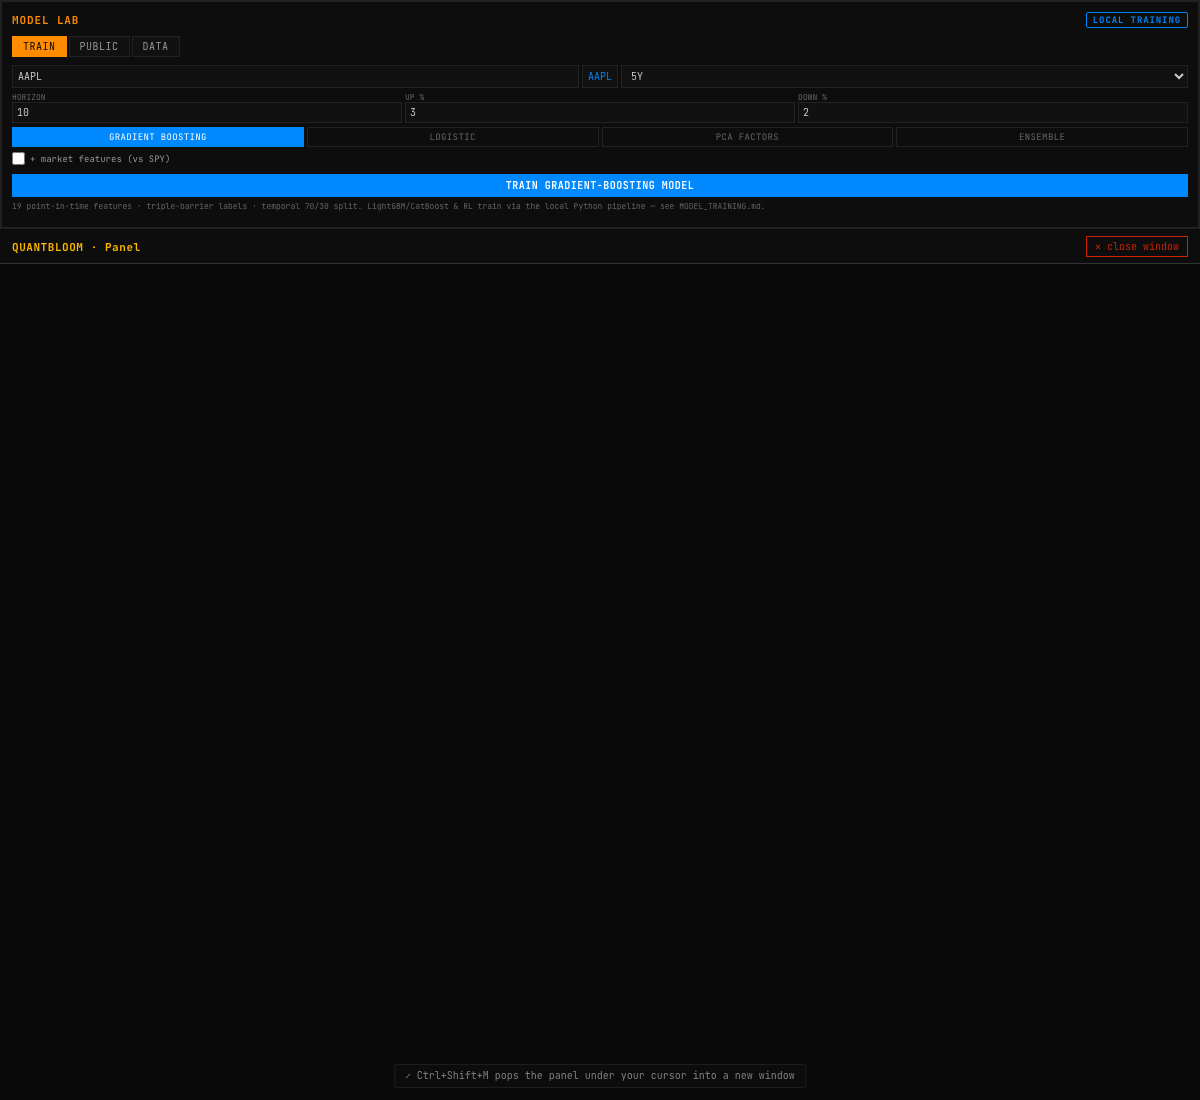
\includegraphics[keepaspectratio,alt={The Model Lab: model-type selector, training controls, out-of-sample metrics, and the publish gate's verdict.}]{img/model-lab.png}}
\caption{The Model Lab: model-type selector, training controls,
out-of-sample metrics, and the publish gate's verdict.}
\end{figure}

\emph{Figure 4. The Model Lab --- train a model, read its out-of-sample
metrics, and see the publish gate's decision.}

\subsubsection{6.1 Regularised logistic
regression}\label{regularised-logistic-regression}

The baseline model predicts \(P(y=1\mid x) = \sigma(w^\top z + b)\)
where \(\sigma(a) = 1/(1+e^{-a})\) and \(z\) is the standardised feature
vector \(z_j = (x_j - \mu_j)/\sigma_j\) (the scaler is stored with the
model). Training minimises the L2-regularised cross-entropy

\[
\mathcal{L}(w,b) = -\frac{1}{N}\sum_{i=1}^{N}\Big[y_i\log p_i + (1-y_i)\log(1-p_i)\Big] + \frac{\lambda}{2}\lVert w\rVert^2
\]

by batch gradient descent, using the standard logistic gradient
\(\nabla_w \mathcal{L} = \tfrac{1}{N}\sum_i (p_i - y_i)\,z_i + \lambda w\).
It is a transparent, low-variance baseline; any more complex model has
to beat it.

\subsubsection{6.2 Gradient-boosted decision
trees}\label{gradient-boosted-decision-trees}

\texttt{bot/gbm.js} implements Friedman's gradient boosting as the
in-app stand-in for LightGBM/CatBoost. It fits an additive model
\(F_M(x) = \sum_{m=1}^{M}\nu\,h_m(x)\) of shallow regression trees to
the \textbf{pseudo-residuals of the log-loss}. Working in logit space
with \(p = \sigma(F)\), the negative gradient of the log-loss at stage
\(m\) is simply

\[
r_i^{(m)} = y_i - \sigma\!\big(F_{m-1}(x_i)\big),
\]

i.e.~the current probability error. Each stage fits a shallow CART
regression tree \(h_m\) to \(\{(x_i, r_i^{(m)})\}\) by exhaustive split
search minimising squared error, with a minimum-leaf-size constraint,
and the ensemble is updated with a learning rate \(\nu\) (shrinkage).
The final prediction is \(\sigma(F_M(x))\). Split-count \textbf{feature
importance} is reported, normalised to sum to one.

The decisive test is that the GBM \textbf{learns XOR} --- a function no
linear model can represent --- achieving accuracy \(>0.85\) where
logistic regression sits near \(0.5\). Building this model also surfaced
a real methodological bug: a naive linear-congruential PRNG produces
serially-correlated ``noise'' that the GBM was powerful enough to learn,
giving fabricated out-of-sample AUC of 0.96; switching to a
\texttt{mulberry32} PRNG with independent feature/label streams restored
the expected \(\approx 0.5\). This is itself a small demonstration of
why the overfitting guards in Section 7 exist.

\subsubsection{6.3 The PCA latent-factor
model}\label{the-pca-latent-factor-model}

The latent-factor family (the in-app, clean-room stand-in for the
ml4t-models PCA/RPPCA/IPCA family) reduces the standardised features to
their top-\(k\) principal components --- the directions of greatest
variance, the ``latent factors'' --- then predicts the label from those
components with logistic regression.

PCA requires the eigenvectors of the feature covariance matrix. Because
a covariance matrix is symmetric, QuantBloom uses a \textbf{from-scratch
cyclic Jacobi eigensolver} (\texttt{bot/eigen.js}). Jacobi repeatedly
applies a plane rotation \(R(p,q,\theta)\) that annihilates the largest
off-diagonal entry:

\[
\theta = \tfrac{1}{2}\operatorname{atan2}\!\big(2a_{pq},\ a_{pp}-a_{qq}\big),\qquad
A \leftarrow R^\top A R,
\]

accumulating \(V \leftarrow VR\) until \(A\) is diagonal; the diagonal
then holds the eigenvalues and the columns of \(V\) the eigenvectors.
The solver is verified against known decompositions, orthonormality,
\(Av=\lambda v\) for every returned pair, and the trace/determinant
identities. PCA (\texttt{bot/pca.js}) standardises \(X\), forms the
covariance from the columns, eigendecomposes it, and projects onto the
top-\(k\) loadings; the fraction of variance explained per component is
reported. On real data, five factors typically capture \(\approx 82\%\)
of feature variance.

\subsubsection{6.4 The ensemble}\label{the-ensemble}

The ensemble averages the predicted probabilities of the GBM, logistic,
and PCA members:
\(\hat p_\text{ens}(x) = \tfrac{1}{3}\big(\hat p_\text{gbm} + \hat p_\text{log} + \hat p_\text{pca}\big)\).
Averaging decorrelated errors trades a little of each model's bias for
lower variance; the test suite asserts the blend is never worse than its
weakest member. As Section 16 records, on real data the ensemble
improves \emph{robustness} but does not beat the best single model, and
--- like every model here --- does not beat buy-and-hold.

\subsubsection{6.5 Evaluation metrics}\label{evaluation-metrics}

\texttt{evaluate()} reports accuracy, precision, recall, F1, and a
rank-based \textbf{AUC} computed via the Mann--Whitney statistic:

\[
\text{AUC} = \frac{1}{|\mathcal{P}||\mathcal{N}|}\sum_{i\in\mathcal{P}}\sum_{j\in\mathcal{N}}\mathbb{1}\big[\hat p_i > \hat p_j\big],
\]

which is threshold-independent and is not fooled by class imbalance the
way raw accuracy is. AUC is the primary discrimination metric in the
publish gate.

\begin{center}\rule{0.5\linewidth}{0.5pt}\end{center}

\subsection{7. Model Evaluation and the Publish
Gate}\label{model-evaluation-and-the-publish-gate}

The single most important design decision in QuantBloom is that a model
cannot reach the public page --- or be trusted --- merely because it
looked good on a backtest. Backtests are optimised over many trials, and
the best of many random strategies will look excellent by chance. The
\textbf{publish gate} (\texttt{bot/model-registry.js},
\texttt{evaluateGate}) enforces a battery of out-of-sample tests,
corrected for multiple testing, before a model is eligible.

\subsubsection{7.1 Risk-adjusted return}\label{risk-adjusted-return}

\texttt{bot/statistics.js} computes the standard summary statistics on
an equity curve. For a return series \(\{r_t\}\) with mean \(\mu\) and
standard deviation \(\sigma\), the annualised \textbf{Sharpe ratio}
(with \(N\) periods per year and risk-free rate \(r_f\)) is

\[
\text{SR} = \frac{\mu - r_f/N}{\sigma}\sqrt{N},
\]

with the \textbf{Sortino ratio} replacing \(\sigma\) by the downside
deviation, and the \textbf{maximum drawdown} the largest peak-to-trough
decline of the cumulative curve.

\subsubsection{7.2 The Probabilistic Sharpe
Ratio}\label{the-probabilistic-sharpe-ratio}

A Sharpe estimate from a finite, non-normal sample is itself uncertain.
The \textbf{Probabilistic Sharpe Ratio} (Bailey \& López de Prado) gives
the probability that the true Sharpe exceeds a benchmark
\(\text{SR}^\star\), correcting for skew \(\gamma_3\) and kurtosis
\(\gamma_4\) and sample length \(n\):

\[
\text{PSR}(\text{SR}^\star) = \Phi\!\left(
\frac{(\widehat{\text{SR}} - \text{SR}^\star)\sqrt{n-1}}
     {\sqrt{\,1 - \gamma_3\widehat{\text{SR}} + \tfrac{\gamma_4-1}{4}\widehat{\text{SR}}^{\,2}\,}}
\right),
\]

where \(\Phi\) is the standard-normal CDF. Fat tails and negative skew
\emph{lower} the PSR: the same point estimate is less trustworthy when
returns are non-normal.

\subsubsection{7.3 The Deflated Sharpe
Ratio}\label{the-deflated-sharpe-ratio}

When a researcher tries \(M\) strategy variants and keeps the best, the
maximum observed Sharpe is inflated purely by selection. The
\textbf{expected maximum Sharpe} under the null (all variants have zero
true edge) is approximated by

\[
\mathbb{E}[\max_M \widehat{\text{SR}}] \approx \sigma_{\text{SR}}\left[(1-\gamma)\,\Phi^{-1}\!\Big(1-\tfrac{1}{M}\Big) + \gamma\,\Phi^{-1}\!\Big(1-\tfrac{1}{Me}\Big)\right],
\]

with \(\gamma\) the Euler--Mascheroni constant and
\(\sigma_{\text{SR}}\) the cross-trial dispersion of Sharpe estimates.
The \textbf{Deflated Sharpe Ratio} is then the PSR benchmarked against
\emph{this} inflated threshold rather than zero:
\(\text{DSR} = \text{PSR}(\mathbb{E}[\max_M \widehat{\text{SR}}])\). A
strategy with a high raw Sharpe but a DSR below \textasciitilde0.90 is
statistically indistinguishable from the luckiest of the variants that
were tried.

\subsubsection{7.4 The Probability of Backtest
Overfitting}\label{the-probability-of-backtest-overfitting}

\texttt{probabilityOfBacktestOverfitting} implements
\textbf{combinatorially-symmetric cross-validation} (CSCV). The
performance matrix (strategies × time slices) is split into all balanced
combinations of in-sample and out-of-sample halves; for each, the
in-sample-best strategy's out-of-sample \textbf{rank} is recorded,
mapped to a logit \(\lambda\), and the PBO is the fraction of
combinations in which the in-sample winner underperforms the
out-of-sample median (\(\lambda < 0\)):

\[
\text{PBO} = \Pr[\lambda < 0].
\]

A PBO above 50\% means selecting the best backtest is \emph{worse} than
a coin flip out of sample --- a direct, model-agnostic measure of
overfitting.

\subsubsection{7.5 The gate}\label{the-gate}

A model is \emph{eligible to publish} only if, on the held-out test
window, it clears \textbf{all} of:

{\def\LTcaptype{none} % do not increment counter
\begin{longtable}[]{@{}lll@{}}
\toprule\noalign{}
Criterion & Threshold & Guards against \\
\midrule\noalign{}
\endhead
\bottomrule\noalign{}
\endlastfoot
Test AUC & \(\ge 0.55\) & no directional edge \\
Out-of-sample Sharpe & \(\ge 0.5\) & poor risk-adjusted return \\
Beats buy-and-hold & required & closet indexing \\
Deflated Sharpe & \(\ge 0.90\) & multiple-testing luck \\
Test trades & \(\ge 5\) & statistically empty backtest \\
Test rows & \(\ge 60\) & too little held-out data \\
\end{longtable}
}

The gate is deliberately demanding. The server re-checks eligibility on
publish, so a client cannot force a model through. Section 16 reports
the honest consequence: no daily-bar model currently clears it.

\begin{center}\rule{0.5\linewidth}{0.5pt}\end{center}

\subsection{8. Backtesting Methodology}\label{backtesting-methodology}

\texttt{bot/backtest.js} is an \textbf{event-driven, point-in-time}
backtester shared in spirit with the live engine. Its correctness rests
on three rules:

\begin{enumerate}
\def\labelenumi{\arabic{enumi}.}
\tightlist
\item
  \textbf{No look-ahead.} At each bar \(t\), signals are computed from
  bars \([0..t]\) only.
\item
  \textbf{Fills at the next bar's open.} A signal generated on the close
  of bar \(t\) fills at \(O_{t+1}\), never at \(C_t\). Filling at the
  signal bar's close is the classic way to fabricate returns; the
  backtester structurally forbids it.
\item
  \textbf{Costs on every fill.} Each fill pays commission (0.5¢/share),
  slippage (5 bps), and half-spread (2 bps). The reported cost drag is
  explicit.
\end{enumerate}

Every run is compared to a \textbf{buy-and-hold} benchmark over the
identical window. \texttt{walkForward} runs rolling train/test folds and
reports the fraction of folds in which the strategy beats buy-and-hold
and the consistency of that outperformance. \texttt{sweepStrategies}
tries many parameter variants and reports the Deflated Sharpe and PBO
\textbf{alongside} the raw numbers, so a user reads the honest picture
rather than the cherry-picked best.

\begin{figure}
\centering
\pandocbounded{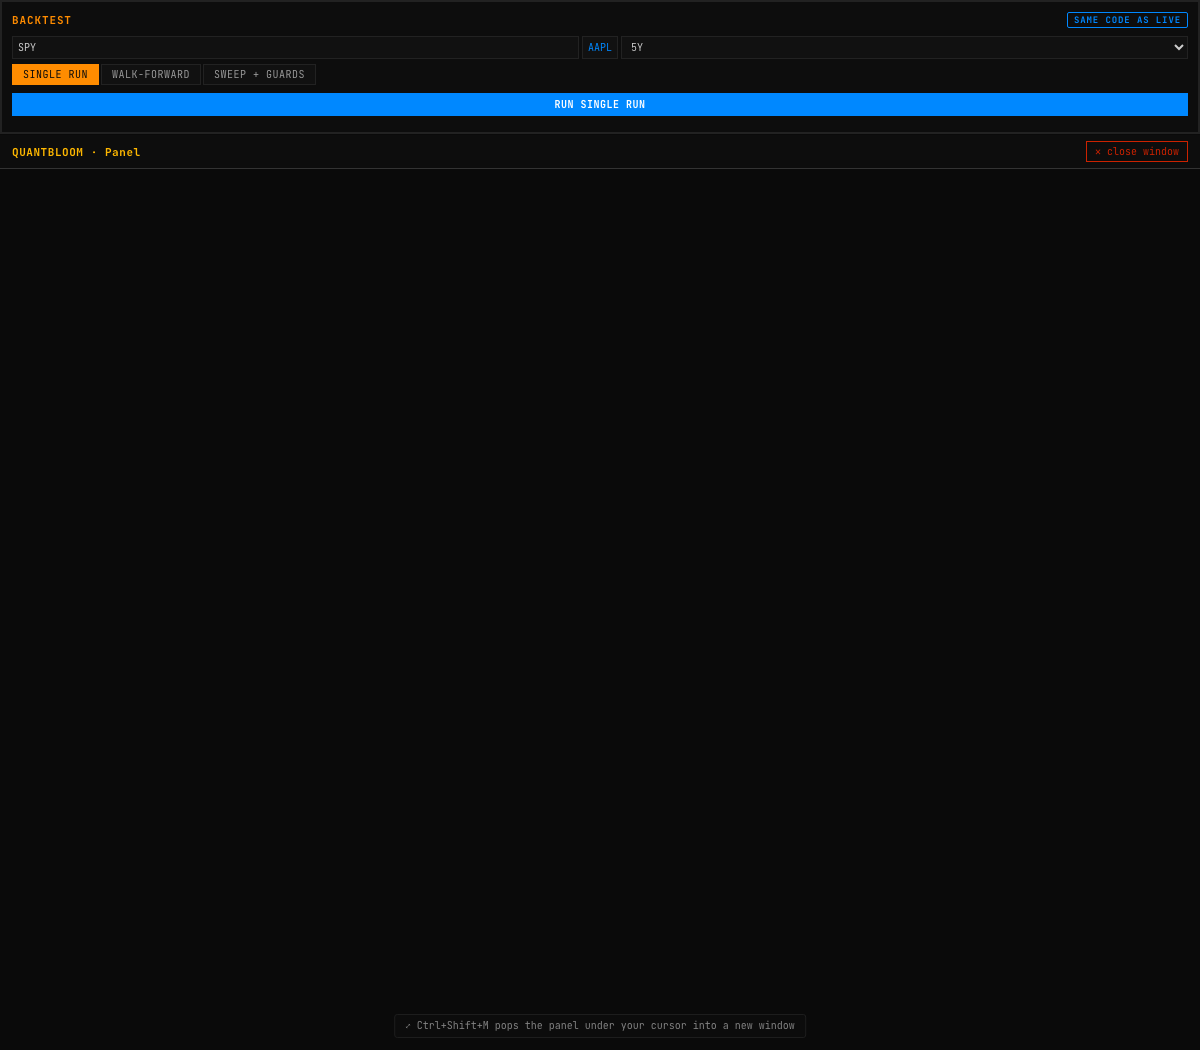
\includegraphics[keepaspectratio,alt={The backtester: strategy vs.~buy-and-hold equity curves, a full metrics table, and the explicit cost drag.}]{img/backtest.png}}
\caption{The backtester: strategy vs.~buy-and-hold equity curves, a full
metrics table, and the explicit cost drag.}
\end{figure}

\emph{Figure 5. A single backtest run --- strategy equity (orange)
against buy-and-hold, with a complete metrics table and the
transaction-cost drag stated in dollars.}

When run on real SPY data, the tooling behaves exactly as it should: a
rule strategy returns +2.2\% against buy-and-hold's +81.6\% over the
window, with a Deflated Sharpe of 0 and a PBO of 65\% --- correctly
reporting \emph{no edge}.

\begin{center}\rule{0.5\linewidth}{0.5pt}\end{center}

\subsection{9. Rule-Based Trading
Strategies}\label{rule-based-trading-strategies}

\texttt{bot/strategies.js} provides six transparent strategies, each
returning the same shape \texttt{\{action,\ confidence,\ rationale\}} so
they compose:

\begin{itemize}
\tightlist
\item
  \textbf{RSI reversion} --- buy oversold (\(\text{RSI}<30\)), sell
  overbought (\(>70\)).
\item
  \textbf{MACD momentum} --- follow the histogram sign, scaled by size
  relative to price.
\item
  \textbf{Trend following} --- the 50/200 golden/death cross confirmed
  by price vs.~the 50-day.
\item
  \textbf{Bollinger reversion} --- fade moves outside the 20/2 bands.
\item
  \textbf{Contrarian} --- the default of the course trader bots: fade
  the latest move, \(\text{position} = -\operatorname{sign}\) of recent
  momentum, using the 12-EMA as the momentum reference.
\item
  \textbf{Indicator consensus} --- the net vote across the twelve
  indicators in the technical engine.
\end{itemize}

An \textbf{ensemble} takes a weighted vote across the enabled
strategies; disagreement shrinks the confidence, and position size is
confidence-proportional. Five \textbf{presets} (conservative, balanced,
aggressive, trend-only, reversion-only) change how much the bot trades
--- pairing the two families that fail in opposite regimes is what keeps
the ensemble mostly still. Each strategy documents its
\texttt{worksWhen} and \texttt{failsWhen} in the UI.

\begin{center}\rule{0.5\linewidth}{0.5pt}\end{center}

\subsection{10. The Trading Bot}\label{the-trading-bot}

The bot (\texttt{bot/engine.js}, \texttt{bot/alpaca.js}) trades a
watchlist against an Alpaca \textbf{paper} account. It is off by default
and every order passes a hard risk gate.

\begin{figure}
\centering
\pandocbounded{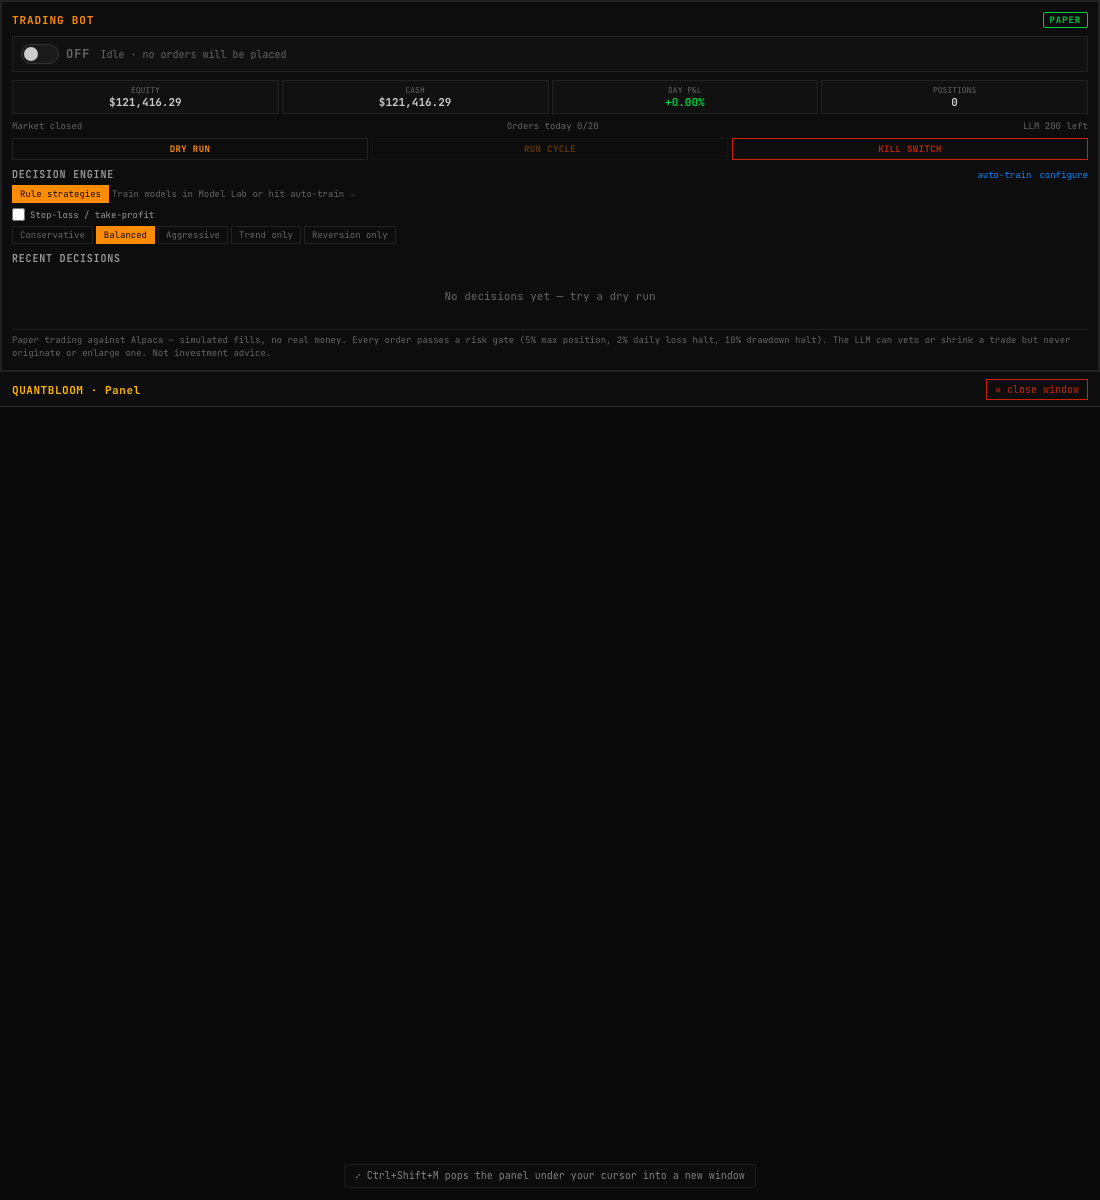
\includegraphics[keepaspectratio,alt={The trading bot: on/off switch, account state, decision engine selector (rule strategies or a trained model), protective-exit controls, and the decision log.}]{img/trading-bot.png}}
\caption{The trading bot: on/off switch, account state, decision engine
selector (rule strategies or a trained model), protective-exit controls,
and the decision log.}
\end{figure}

\emph{Figure 6. The trading bot --- decision-engine selector,
stop-loss/take-profit and trailing controls, and the risk gate at work.}

\subsubsection{10.1 The decision loop}\label{the-decision-loop}

Each cycle fetches account, positions and the market clock; checks halt
conditions; and for each watchlist symbol produces a decision either
from the rule ensemble or --- if one is selected --- from a trained ML
model (\texttt{modelStrategy}). The decision optionally passes through
the LLM advisory layer, then the risk gate, then execution.

\subsubsection{10.2 The risk gate}\label{the-risk-gate}

\texttt{bot/risk-gate.js} is the safety core. Every order passes through
\texttt{evaluateOrder}, which \textbf{clamps rather than rejects} where
it can, enforcing hard ceilings that code --- not configuration ---
guarantees:

\begin{itemize}
\tightlist
\item
  Max \textbf{5\%} of equity per position; max \textbf{25\%} per sector;
  max \textbf{100\%} gross exposure.
\item
  Max \textbf{2\%} daily loss (auto-clears overnight) and max
  \textbf{10\%} drawdown from the high-water mark (requires a manual
  restart).
\item
  Max \textbf{20} orders/day; a liquidity cap of a fraction of 20-day
  ADV; a minimum order value to avoid dust.
\end{itemize}

\texttt{checkHaltConditions} distinguishes a daily-loss halt (temporary)
from a drawdown halt (which requires a deliberate restart), so a bad day
cannot silently resume into a bad week.

\subsubsection{10.3 Position sizing}\label{position-sizing}

Size is confidence-proportional, bounded by the position ceiling:
\(q = \big\lfloor \tfrac{E\cdot m\cdot \max(c,\,c_{\min})}{P} \big\rfloor\)
where \(E\) is equity, \(m\) the max-position fraction, \(c\) the
decision confidence, and \(P\) the price.

\subsubsection{10.4 Protective exits}\label{protective-exits}

\texttt{bot/brackets.js} computes tick-rounded stop-loss and take-profit
prices for a long entry (\(\text{stop} < \text{entry} < \text{target}\))
and submits them as an Alpaca \textbf{bracket order}, so the exits are
managed broker-side and fire even if the bot process is down.
Percentages are capped (stop \(\le 50\%\), target \(\le 200\%\)) so a
fat-finger cannot disarm the protection. A \textbf{live trailing stop}
ratchets a per-symbol high-water mark each cycle and forces an exit when
price falls the trail distance below the peak; it runs \emph{after} the
LLM review so a protective stop can never be vetoed.

\subsubsection{10.5 The kill switch and
self-training}\label{the-kill-switch-and-self-training}

The \textbf{kill switch} disables the bot, cancels working orders,
flattens all positions, and requires a manual restart.
\textbf{Auto-train} trains a model on every watchlist symbol and
auto-selects the strongest --- preferring one that clears the publish
gate, else the best out-of-sample AUC --- and honestly reports ``none
worth using'' when nothing qualifies.

\begin{center}\rule{0.5\linewidth}{0.5pt}\end{center}

\subsection{11. The LLM Advisory Layer}\label{the-llm-advisory-layer}

\texttt{bot/mistral.js} adds a Mistral LLM as a strictly
\textbf{advisory} reviewer. It sees a decision the quantitative layers
already made and returns a structured stance (\texttt{AGREE} /
\texttt{DISAGREE} / \texttt{CAUTION}) with confidence and a stated key
risk. Its influence is one-directional --- toward doing \emph{less}: a
confident \texttt{DISAGREE} vetoes the trade (forces \texttt{HOLD}); a
\texttt{CAUTION} or weak \texttt{DISAGREE} halves the confidence (and
thus the size). It can never originate a trade, flip a direction, or
increase size. Every call is logged with its full response, a daily
budget cap is enforced, and the layer degrades to a no-op when
unavailable. This containment is deliberate: the LLM's qualitative
context (an earnings event, a news shock) is valuable, but its failure
modes --- non-determinism, confident nonsense --- are neutralised by
giving it no execution authority.

\begin{center}\rule{0.5\linewidth}{0.5pt}\end{center}

\subsection{12. Portfolio and Valuation
Analytics}\label{portfolio-and-valuation-analytics}

\subsubsection{12.1 Mean-variance
optimisation}\label{mean-variance-optimisation}

\texttt{portfolio-math.js} implements Markowitz optimisation in closed
form via \textbf{two-fund separation}. Given the covariance matrix
\(\Sigma\) and mean-return vector \(\mu\), with \(\mathbf{1}\) the ones
vector, define \(A = \mathbf{1}^\top\Sigma^{-1}\mathbf{1}\),
\(B = \mathbf{1}^\top\Sigma^{-1}\mu\), \(C = \mu^\top\Sigma^{-1}\mu\).
The \textbf{global minimum-variance} portfolio is

\[
w_{\text{mv}} = \frac{\Sigma^{-1}\mathbf{1}}{A},
\]

and every frontier portfolio is a combination of \(w_{\text{mv}}\) and a
second efficient fund. The efficient frontier is traced by sweeping the
risk-aversion parameter \(\lambda \ge 0\) (clamped non-negative so the
lower, dominated branch of the hyperbola is excluded --- a bug the
monotonicity test caught early). The \textbf{tangency} (max-Sharpe)
portfolio maximises \((w^\top\mu - r_f)/\sqrt{w^\top\Sigma w}\).

\begin{figure}
\centering
\pandocbounded{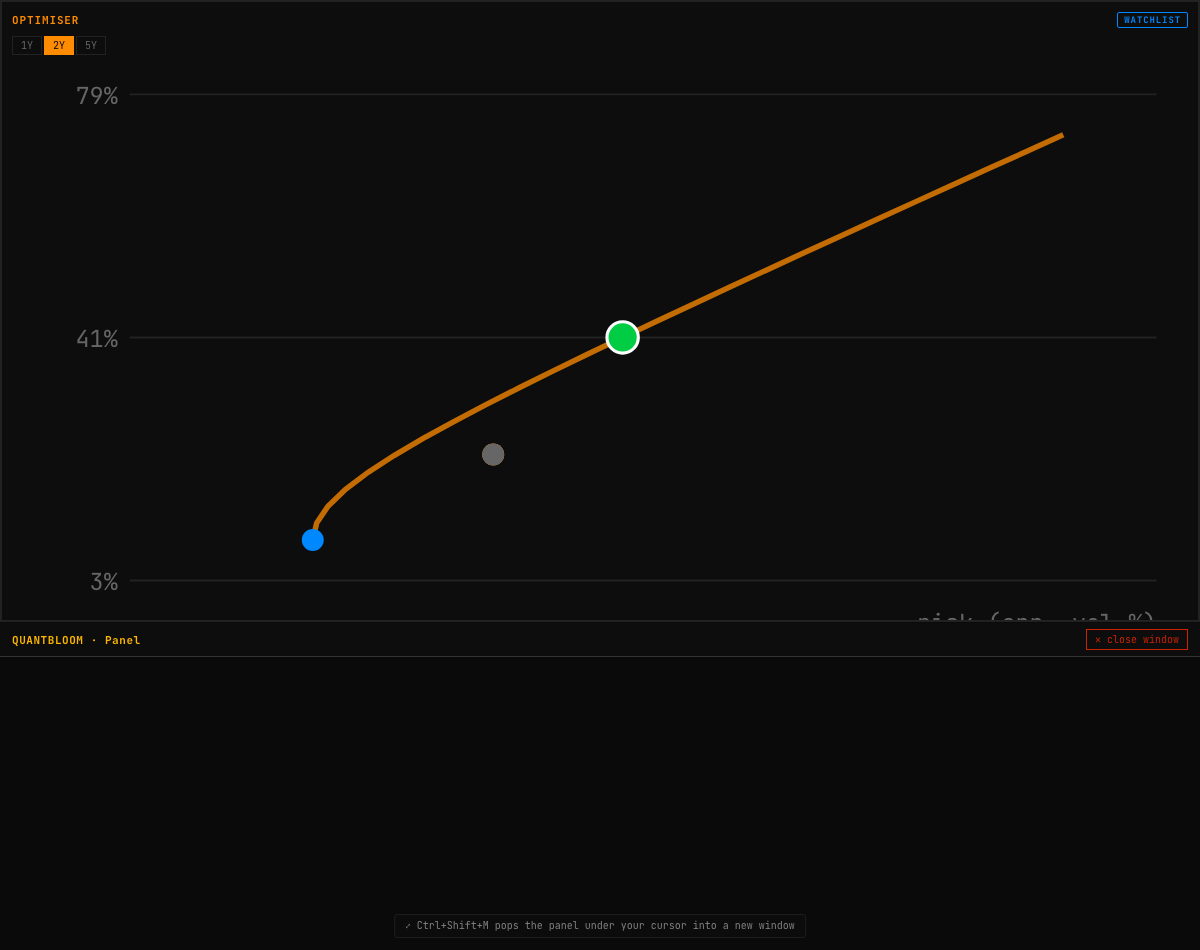
\includegraphics[keepaspectratio,alt={The optimiser: the efficient frontier with the minimum-variance and max-Sharpe portfolios against the current allocation.}]{img/optimiser.png}}
\caption{The optimiser: the efficient frontier with the minimum-variance
and max-Sharpe portfolios against the current allocation.}
\end{figure}

\emph{Figure 7. Portfolio optimisation --- the efficient frontier and
the special portfolios, labelled clearly as a historical-input model.}

\subsubsection{12.2 Value at Risk}\label{value-at-risk}

The VaR panel computes 95\%/99\% VaR and Conditional VaR (expected
shortfall) by \textbf{three methods} whose disagreement is itself
informative:

\begin{itemize}
\tightlist
\item
  \textbf{Historical} --- the empirical quantile of realised returns.
\item
  \textbf{Parametric} ---
  \(\text{VaR}_\alpha = -(\mu + z_\alpha\sigma)\,V\) under normality,
  with \(z_\alpha\) the standard-normal quantile.
\item
  \textbf{Monte Carlo} --- simulated draws from the fitted distribution.
\end{itemize}

Fat tails show up precisely as historical VaR exceeding parametric VaR;
CVaR (the mean loss beyond the VaR threshold) captures the tail the
quantile omits.

\begin{figure}
\centering
\pandocbounded{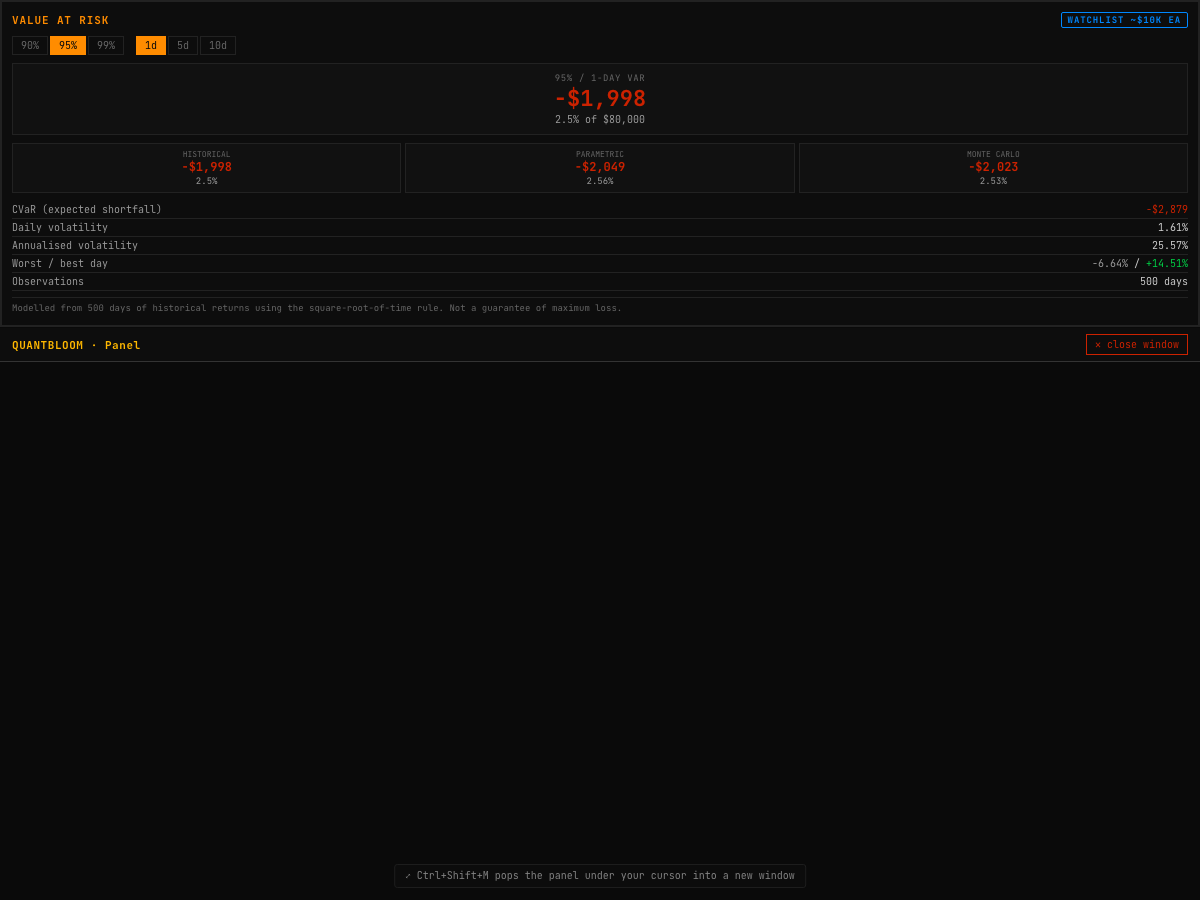
\includegraphics[keepaspectratio,alt={Value at Risk by three methods, with CVaR and the volatility diagnostics.}]{img/value-at-risk.png}}
\caption{Value at Risk by three methods, with CVaR and the volatility
diagnostics.}
\end{figure}

\emph{Figure 8. Three-method VaR --- historical, parametric, and
Monte-Carlo --- with Conditional VaR and volatility, modelled from the
return history.}

\subsubsection{12.3 Factor exposure}\label{factor-exposure}

\texttt{regression.js} provides multiple OLS regression with
\(p\)-values. The factor panel regresses portfolio returns on
Fama--French-style factor proxies (market, size, value, momentum via
representative ETFs),

\[
r_p = \alpha + \sum_k \beta_k f_k + \varepsilon,
\]

to reveal unintended style tilts; each loading is reported with its
significance.

\begin{figure}
\centering
\pandocbounded{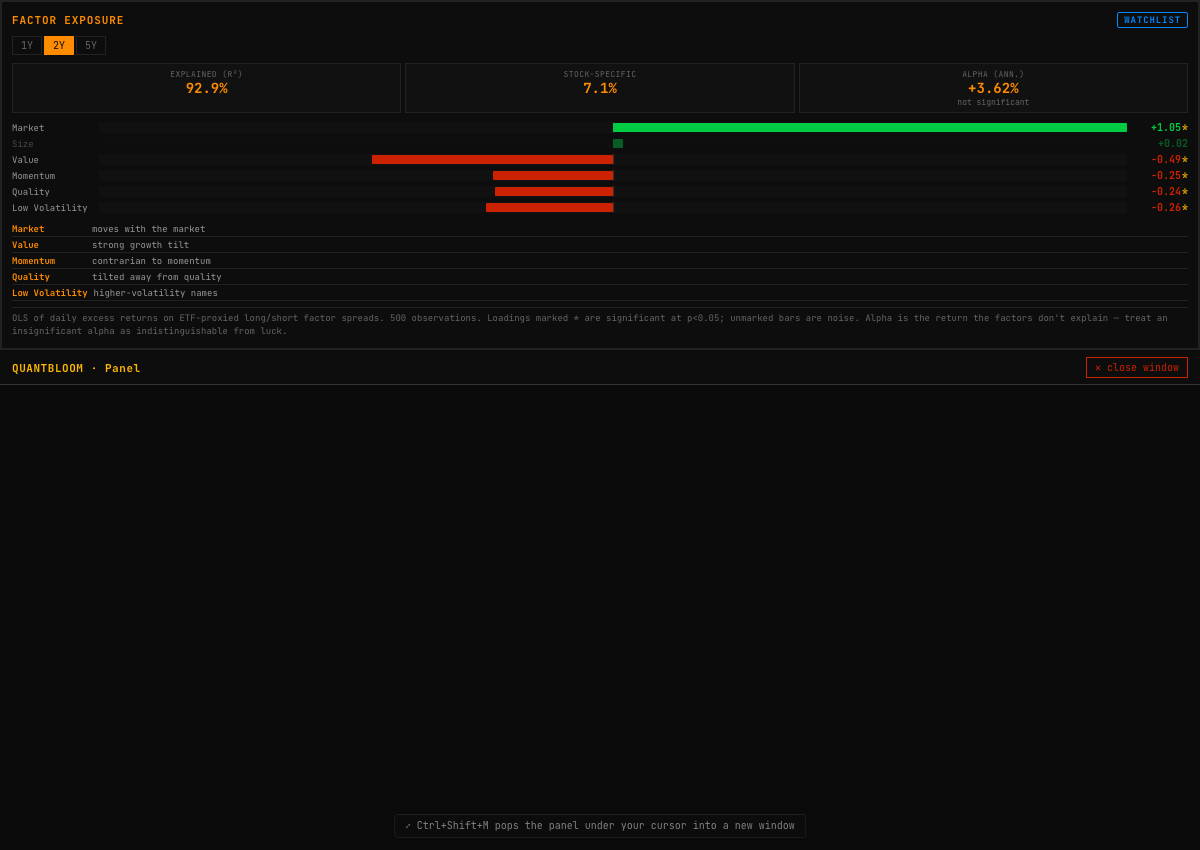
\includegraphics[keepaspectratio,alt={Factor exposure --- regression loadings on the market, size, value, and momentum factors.}]{img/factor-exposure.png}}
\caption{Factor exposure --- regression loadings on the market, size,
value, and momentum factors.}
\end{figure}

\emph{Figure 9. Factor regression --- the portfolio's style tilts and
their significance.}

\subsubsection{12.4 DCF valuation and time value of
money}\label{dcf-valuation-and-time-value-of-money}

The DCF panel discounts projected free cash flows with a Gordon-growth
terminal value and a WACC × terminal-growth sensitivity grid, producing
an intrinsic value against market price --- labelled, emphatically, as a
model only as good as its inputs.

\begin{figure}
\centering
\pandocbounded{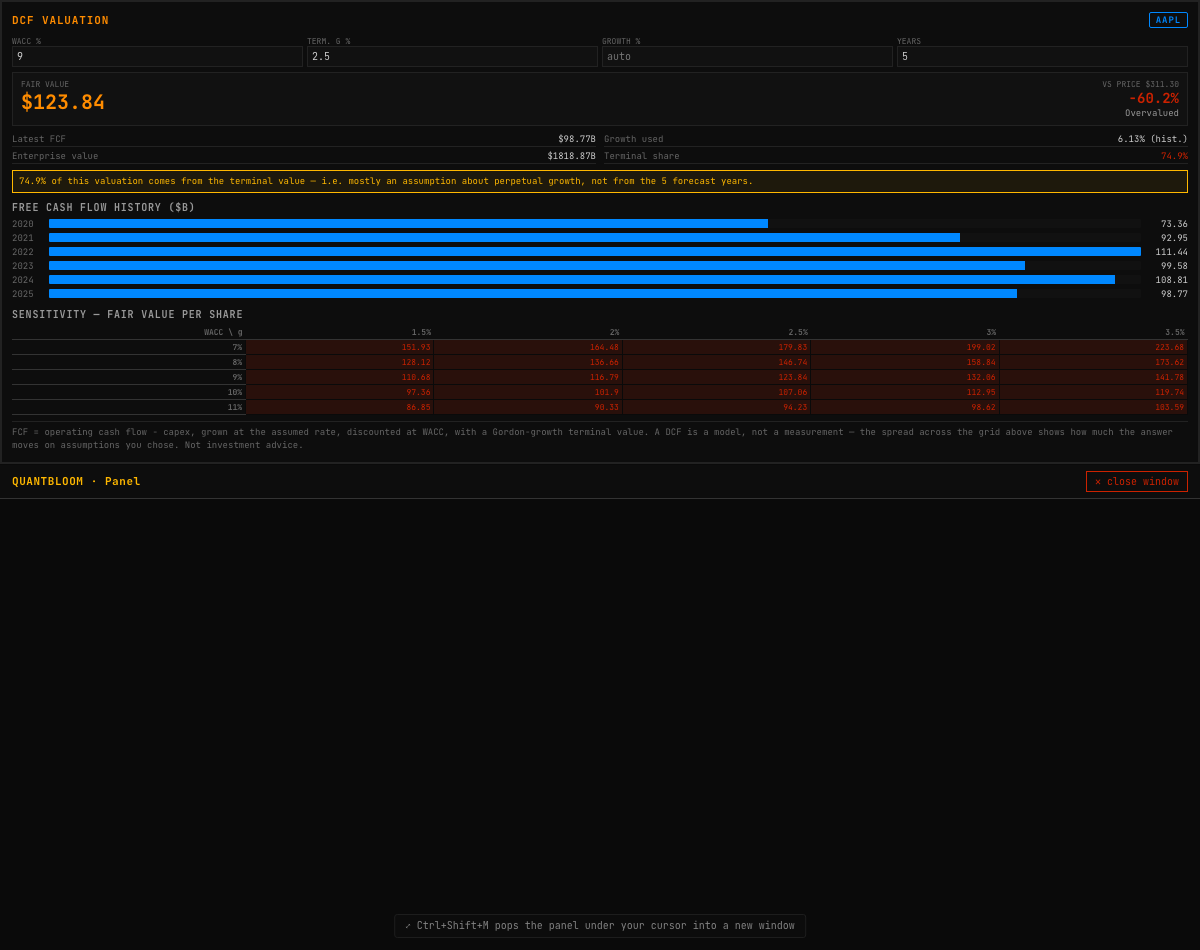
\includegraphics[keepaspectratio,alt={Discounted cash-flow valuation with an editable assumption set and a sensitivity grid.}]{img/dcf.png}}
\caption{Discounted cash-flow valuation with an editable assumption set
and a sensitivity grid.}
\end{figure}

\emph{Figure 10. DCF valuation --- intrinsic value with a WACC ×
terminal-growth sensitivity table.}

The \textbf{time-value-of-money} calculator (\texttt{bot/tvm.js})
implements present/future value with compounding frequency \(m\),
\(\text{FV} = \text{PV}\,(1 + r/m)^{nm}\); net present value
\(\text{NPV} = \sum_i \text{CF}_i/(1+r)^i\); internal rate of return by
Newton--Raphson with a bisection fallback; nominal/effective rate
conversion; and level annuities. Its tests use the source course's own
worked answers as the oracle --- a \$1\{,\}000 payment discounted at 5\%
over 10 years is \$613.9133 annually and \$607.1610 monthly.

\begin{center}\rule{0.5\linewidth}{0.5pt}\end{center}

\subsection{13. The Power \& Commodities
Desk}\label{the-power-commodities-desk}

A distinctive addition, derived from a Citadel power \& gas primer
(\emph{``Power 2026: Electricity Pricing in the Age of AI''}), is a
wholesale-electricity pricing desk (\texttt{charting/power.js}).
Wholesale power clears by \textbf{marginal-cost (merit-order) pricing},
which reduces to small, deterministic computations.

\begin{figure}
\centering
\pandocbounded{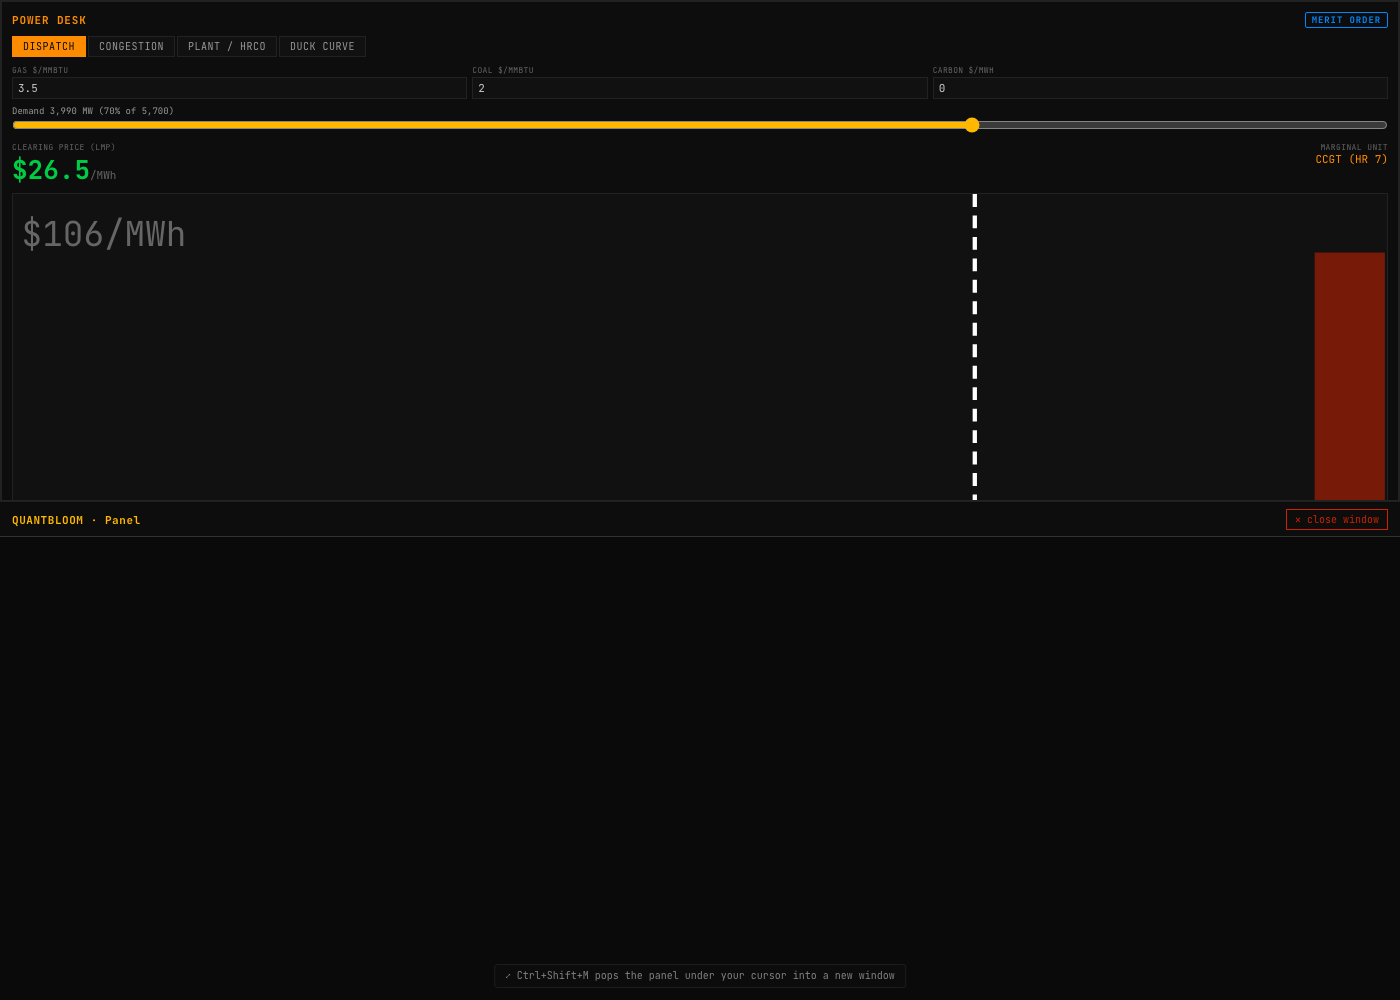
\includegraphics[keepaspectratio,alt={The Power Desk --- a merit-order supply stack with the clearing price, the marginal unit, and the demand cut.}]{img/power-desk.png}}
\caption{The Power Desk --- a merit-order supply stack with the clearing
price, the marginal unit, and the demand cut.}
\end{figure}

\emph{Figure 11. The Power Desk --- the merit-order supply stack; the
dashed line is demand, the marginal unit sets the clearing price.}

\subsubsection{13.1 Merit-order dispatch and marginal
pricing}\label{merit-order-dispatch-and-marginal-pricing}

Generators are ranked cheapest-first and dispatched to meet demand; the
last unit needed --- the \textbf{marginal unit} --- sets a single
uniform clearing price that \emph{every} dispatched unit is paid. A
cheaper unit therefore earns \textbf{inframarginal rent} equal to
(clearing price − its own cost) × MW, while the marginal unit earns
zero. The marginal cost of a thermal unit is
\(\text{MC} = \text{HeatRate}\times \text{FuelPrice} + \text{VOM} + \text{Carbon}\),
so a change in the gas price re-orders the stack (fuel switching). The
tests assert cheapest-first dispatch, that pushing demand past a cheap
unit raises the price to the next unit, and that production cost sums
own-cost (not the clearing price).

\subsubsection{13.2 Two-node locational marginal
pricing}\label{two-node-locational-marginal-pricing}

With a transmission line of finite capacity between two buses, the
cheaper node exports its spare capacity up to the line limit. While the
line has slack, one price clears both nodes; the moment it
\textbf{saturates} and the dearer node must self-supply, the prices
\textbf{decouple} --- the exporter clears at its low cost, the importer
at its high cost. That gap is the \textbf{congestion basis}, the payoff
of a Financial Transmission Right. The implementation reproduces the
primer's example exactly: 10 MW over a 50 MW line clears both nodes at
\$10; 60 MW pins the line and decouples to \$100 / \$10 (a \$90 basis);
widening the line re-couples the price.

\begin{figure}
\centering
\pandocbounded{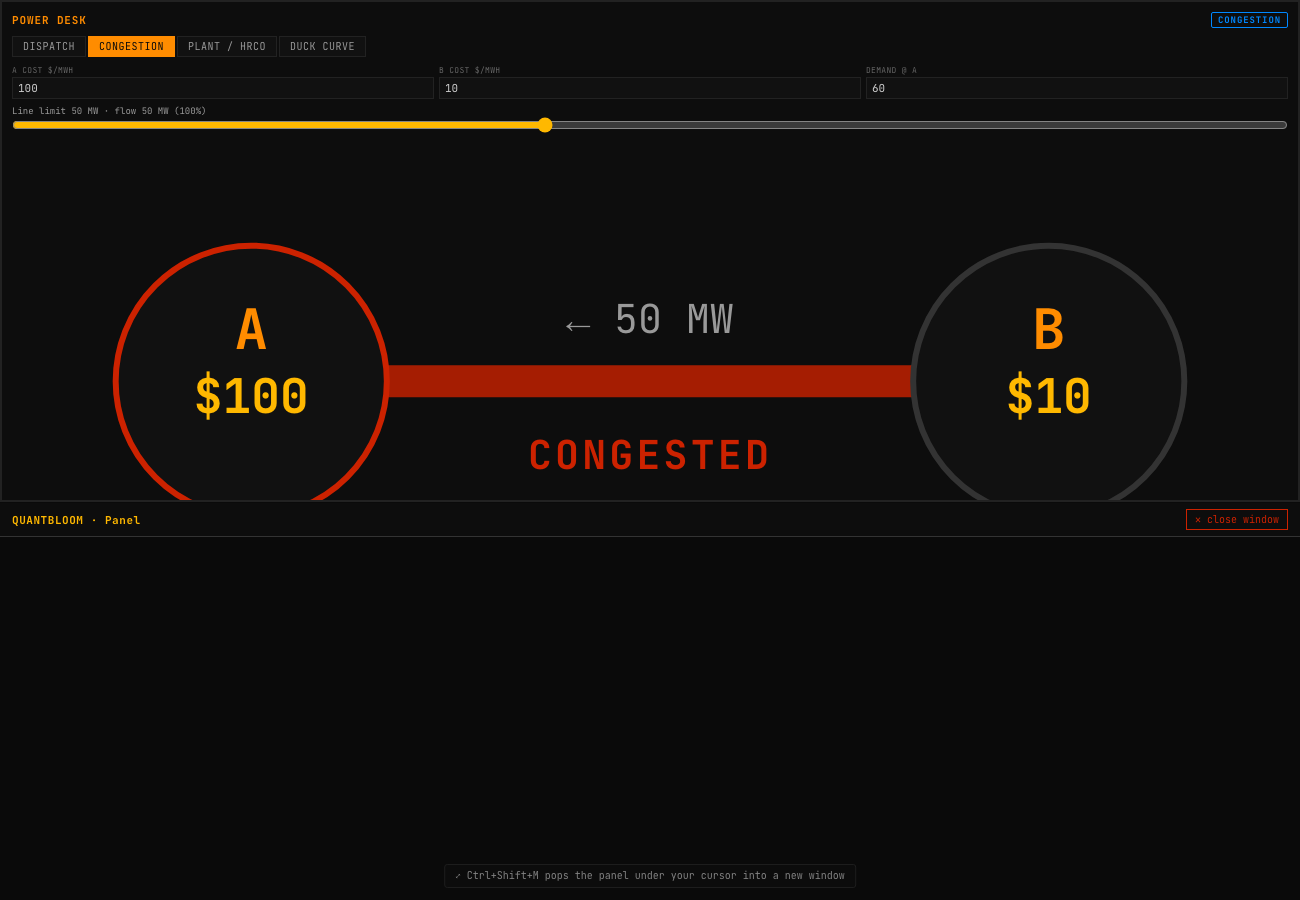
\includegraphics[keepaspectratio,alt={Two-node LMP under congestion: with 60 MW of demand at A and a 50 MW line, the line saturates and the prices decouple to \$100 (A) and \$10 (B).}]{img/power-congestion.png}}
\caption{Two-node LMP under congestion: with 60 MW of demand at A and a
50 MW line, the line saturates and the prices decouple to \$100 (A) and
\$10 (B).}
\end{figure}

\emph{Figure 13. Transmission congestion --- the line is pinned at its
50 MW limit, so node A's price jumps to its local cost while node B
stays cheap. The gap is the congestion basis.}

\subsubsection{13.3 Spark spreads and the heat-rate call
option}\label{spark-spreads-and-the-heat-rate-call-option}

The \textbf{spark spread} is a gas plant's gross margin,
\(\text{spark} = \text{Power} - \text{HeatRate}\times\text{Gas}\) (the
\textbf{dark spread} is the coal analogue), and the \textbf{effective
(break-even) heat rate} \(\text{HR}^\star = \text{Power}/\text{Gas}\) is
the efficiency at which a unit makes zero margin. A \textbf{heat-rate
call option} monetises a plant's optionality --- it pays the positive
spark day by day. QuantBloom values it by Monte Carlo on correlated
lognormal power and gas paths with martingale drift; by convexity the
option value is at least its intrinsic value, rises with volatility, and
falls as power and gas co-move (a tighter spread). All four properties
are asserted in the test suite.

\subsubsection{13.4 The duck curve and scarcity
pricing}\label{the-duck-curve-and-scarcity-pricing}

Net demand (demand minus renewables) develops a midday trough and an
evening spike as solar penetration grows --- the \textbf{duck curve} ---
which forces less efficient units on in the evening and steepens the
intraday price shape. Energy-only markets add a \textbf{scarcity adder}
of VOLL × P(lost load) on top of the marginal energy price when supply
runs short. Both are provided as interactive, clearly-labelled stylised
models --- QuantBloom has no live ISO/LMP feed, and says so.

\begin{figure}
\centering
\pandocbounded{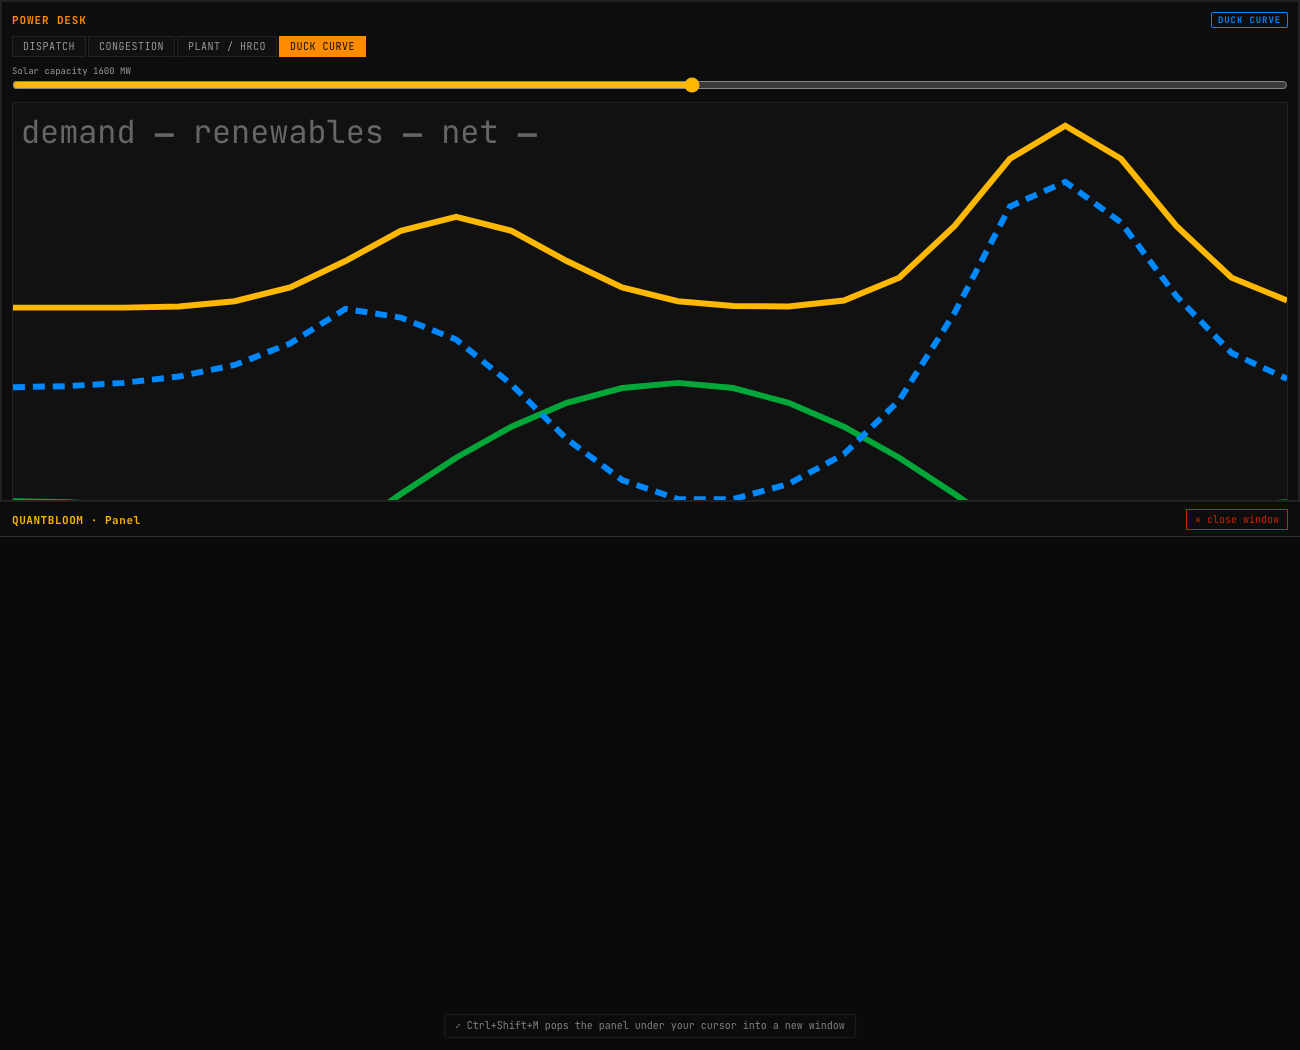
\includegraphics[keepaspectratio,alt={The duck curve --- demand, renewables and net demand over 24 hours, with the resulting evening price spike, on/off-peak strips and a scarcity-adder calculator.}]{img/power-duck.png}}
\caption{The duck curve --- demand, renewables and net demand over 24
hours, with the resulting evening price spike, on/off-peak strips and a
scarcity-adder calculator.}
\end{figure}

\emph{Figure 14. The duck curve --- as solar (green) grows, net demand
(blue) develops a midday belly and an evening neck, steepening the
intraday price shape.}

\begin{center}\rule{0.5\linewidth}{0.5pt}\end{center}

\subsection{14. User Experience and
Workflow}\label{user-experience-and-workflow}

Two Bloomberg-signature interactions make the 37-panel terminal
navigable:

\begin{itemize}
\tightlist
\item
  \textbf{Command palette (\texttt{Ctrl+K}).} The
  \texttt{TICKER\ \textless{}GO\textgreater{}} pattern: one box in which
  a ticker sets the active symbol across every panel, or a panel name
  jumps to it with a highlight flash. The parsing and ranking
  (\texttt{src/lib/command.js}) are pure and tested --- a short alpha
  token is treated as a ticker; an exact panel-title match outranks the
  symbol command.
\item
  \textbf{Panel pop-out (\texttt{Ctrl+Shift+M}).} Any panel opens in its
  own live browser window --- the terminal navigates to
  \texttt{?solo=\textless{}index\textgreater{}}, and a fresh app
  instance focuses that one panel full-window --- so panels can be
  spread across monitors, each fully interactive with its own data.
  (Every figure in this paper was captured through exactly this
  mechanism.)
\end{itemize}

Authentication is optional and Bloomberg-style: with Supabase
configured, access is gated behind a login screen and each signed-in
user is mirrored to a Neon Postgres table; with it unconfigured, the
terminal runs open. A Help \& Shortcuts panel documents the interactions
on-platform.

\begin{figure}
\centering
\pandocbounded{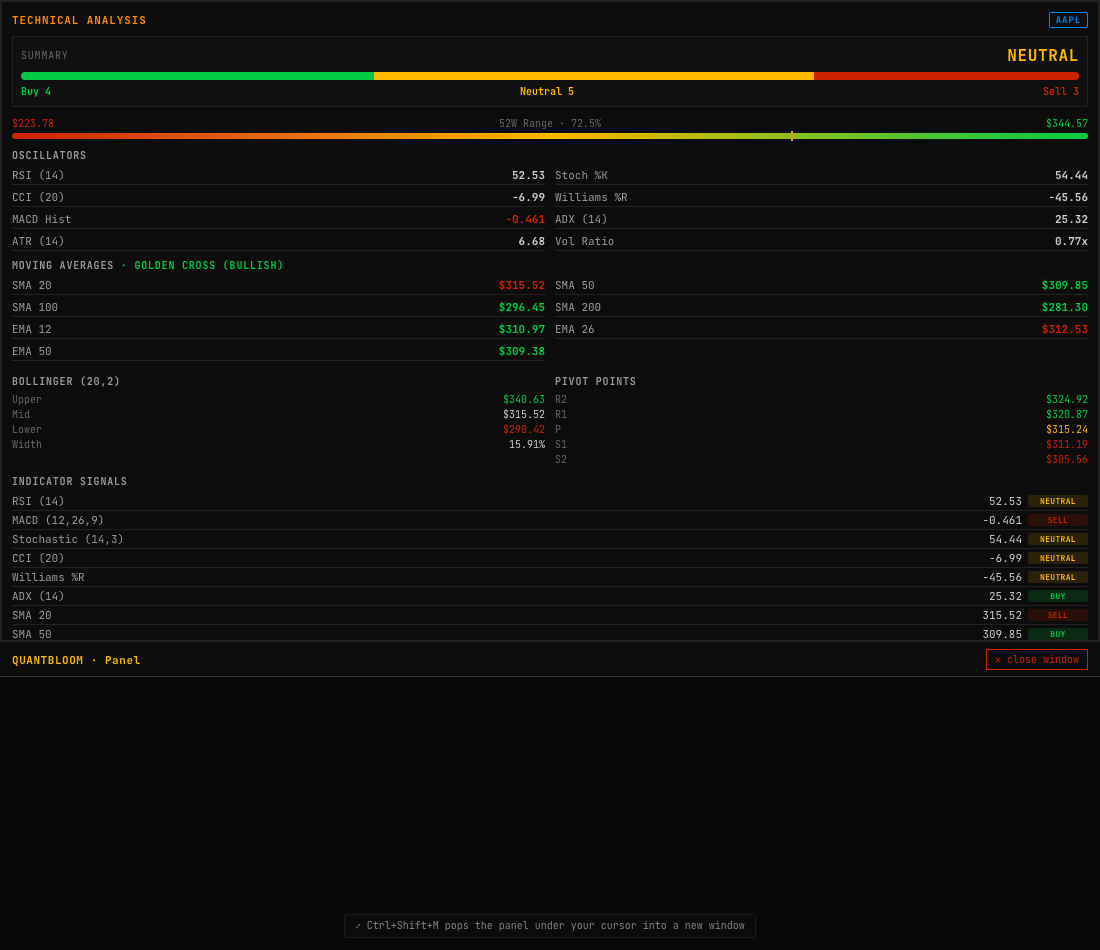
\includegraphics[keepaspectratio,alt={Technical analysis --- twelve indicators with signal scoring and a consolidated verdict.}]{img/technical.png}}
\caption{Technical analysis --- twelve indicators with signal scoring
and a consolidated verdict.}
\end{figure}

\emph{Figure 12. The technical-analysis panel --- twelve indicators,
each scored, rolled into an overall signal.}

\begin{center}\rule{0.5\linewidth}{0.5pt}\end{center}

\subsection{15. Testing and Validation}\label{testing-and-validation}

At the time of writing the repository carries \textbf{332 passing unit
tests} run by the Node built-in test runner (\texttt{node\ -\/-test}).
The philosophy is to assert \emph{defining properties} rather than
fixtures: the GBM must crack XOR; \texttt{sliceUpTo} must never leak a
future bar; the eigensolver must satisfy \(Av=\lambda v\); the formula
sandbox must reject \texttt{constructor}/\texttt{window}/\texttt{eval};
the two-node model must reproduce the primer's \$100/\$10 decoupling;
the TVM functions must match the source's worked answers to the cent;
the merit-order price must jump to the next unit when a cheap unit
saturates. Where a computation is deterministic, the test pins the exact
number; where it is stochastic, a fixed seed makes it reproducible.
Numerically load-bearing changes are verified in the browser (the
production bundle, served by \texttt{node\ server.js}) before they are
committed.

\begin{center}\rule{0.5\linewidth}{0.5pt}\end{center}

\subsection{16. Honest Limitations}\label{honest-limitations}

QuantBloom is built to tell the truth, and the most important truth is
about its own models:

\begin{itemize}
\tightlist
\item
  \textbf{The models do not beat buy-and-hold.} The best daily-bar model
  reaches a test AUC of roughly 0.59 --- genuine but small
  discrimination --- and none clears the publish gate. Long-only
  market-timing of a bull market with a strategy that is often in cash
  cannot beat simply holding the index. The ensemble improves
  robustness, not edge; cross-asset (SPY-relative) features help a
  high-beta name like NVDA (AUC \(0.52 \to 0.56\)) but are noise for
  others. This is the honest reality of daily-bar technical analysis on
  liquid names, and the publish gate is designed to report it rather
  than hide it. \textbf{We did not weaken the gate to manufacture a
  pass.}
\item
  \textbf{No live LMP or Level-2 feed.} The power desk, VaR, DCF, and
  TVM panels are \emph{calculators and stylised models}, not live grid
  or order-book data. They are labelled as such throughout.
\item
  \textbf{Daily bars.} The signal pipeline runs on daily OHLCV. The most
  credible path to genuine edge --- per the source materials --- is
  finer granularity (intraday bars), alternative data, or a different
  objective (confidence-weighted sizing rather than binary direction),
  not more model families on the same 19 features.
\item
  \textbf{Paper trading only.} The bot targets an Alpaca paper endpoint
  by default; \texttt{isPaperEndpoint()} asserts it. Nothing here is
  investment advice.
\end{itemize}

\begin{center}\rule{0.5\linewidth}{0.5pt}\end{center}

\subsection{17. Conclusion and Future
Work}\label{conclusion-and-future-work}

QuantBloom Terminal demonstrates that a rigorous, honest quantitative
research and trading environment can be built entirely in the browser,
with every load-bearing number backed by a tested module. Its
contributions are less any single model than the \emph{discipline}
around them: point-in-time features with enforced train/live parity, a
backtester that structurally forbids look-ahead, and a publish gate that
corrects for multiple testing and refuses to endorse a model that cannot
beat buy-and-hold out of sample.

Natural next steps follow directly from Section 16 and the roadmap:
intraday-bar research; a cross-asset monitor board and an options
volatility surface to round out Bloomberg parity; a live ISO/LMP
integration to turn the power desk's calculators into a live desk; and
the local Python pipeline (documented in \texttt{MODEL\_TRAINING.md})
for the heavier model families (LSTM/CAE/SDF) that cannot run in the
Node runtime, imported back through the same artifact contract and the
same unforgiving publish gate.

\begin{center}\rule{0.5\linewidth}{0.5pt}\end{center}

\subsubsection{Appendix A --- Notation}\label{appendix-a-notation}

{\def\LTcaptype{none} % do not increment counter
\begin{longtable}[]{@{}
  >{\raggedright\arraybackslash}p{(\linewidth - 2\tabcolsep) * \real{0.5000}}
  >{\raggedright\arraybackslash}p{(\linewidth - 2\tabcolsep) * \real{0.5000}}@{}}
\toprule\noalign{}
\begin{minipage}[b]{\linewidth}\raggedright
Symbol
\end{minipage} & \begin{minipage}[b]{\linewidth}\raggedright
Meaning
\end{minipage} \\
\midrule\noalign{}
\endhead
\bottomrule\noalign{}
\endlastfoot
\(P_t, O_t, H_t, L_t, C_t\) & price / open / high / low / close at bar
\(t\) \\
\(r_t\) & period return \\
\(\sigma(\cdot)\) & logistic sigmoid \\
\(z\) & standardised feature vector \\
\(\Sigma, \mu\) & covariance matrix, mean-return vector \\
\(\text{SR}, \text{PSR}, \text{DSR}\) & Sharpe, Probabilistic, Deflated
Sharpe \\
\(\text{PBO}\) & Probability of Backtest Overfitting \\
\(\text{LMP}\) & locational marginal price \\
\(u, d, h\) & triple-barrier up / down / horizon \\
\end{longtable}
}

\subsubsection{Appendix B --- Module and Test
Index}\label{appendix-b-module-and-test-index}

See the table in Section 2.2. Every listed module has a dedicated test
file; the full suite is run with \texttt{npm\ test}
(\texttt{node\ -\/-test\ "test/*.test.mjs"}).

\subsubsection{Appendix C --- A Worked Example: NVDA Through the
Pipeline}\label{appendix-c-a-worked-example-nvda-through-the-pipeline}

To make the abstractions concrete, this appendix traces a single symbol
through the full research pipeline with the actual numbers the system
produces.

\textbf{Step 1 --- Data.} Five years of daily NVDA candles are pulled
from Yahoo (no key). With a 200-bar warm-up and a 10-bar label horizon,
roughly 1,000 labelled rows survive.

\textbf{Step 2 --- Features.} Each surviving bar becomes a
19-dimensional point-in-time vector (Section 5.1). Enabling the
cross-asset option (Section 5.2) aligns SPY to NVDA's bar times and
appends five market-relative features, widening the vector to 24 and
flagging the model \texttt{usesMarket} so the live path knows to supply
the benchmark.

\textbf{Step 3 --- Labelling.} Each row is labelled by the triple
barrier (Section 5.3): \(+3\%\) up, \(-2\%\) down, 10-bar horizon. The
dataset is split temporally, the most recent 30\% held out and never
shuffled.

\textbf{Step 4 --- Training.} A gradient-boosted model (80 trees, depth
3, learning rate 0.08, minimum leaf 15) is fit on the training split. It
reports split-count feature importance; on NVDA the top drivers are
typically volume ratio, MACD histogram, and short-horizon return.

\textbf{Step 5 --- Metrics.} On the held-out window, the model reaches a
\textbf{test AUC of about 0.59} with the base features. Adding the
cross-asset features lifts a high-beta name like NVDA to
\textbf{\textasciitilde0.56--0.62} depending on the window --- genuine
but modest discrimination. The logistic baseline sits near 0.50; PCA
near 0.44--0.52; the ensemble lands between its members.

\textbf{Step 6 --- Out-of-sample backtest.} The model is turned into a
strategy (\texttt{modelStrategy}) and backtested over the test window
with point-in-time signals, next-bar-open fills, and full costs. The
strategy is compared to buy-and-hold; its Deflated Sharpe and trade
count are computed.

\textbf{Step 7 --- The gate.} The publish gate (Section 7.5) checks AUC
\(\ge 0.55\), OOS Sharpe \(\ge 0.5\), beat buy-and-hold, Deflated Sharpe
\(\ge 0.90\), \(\ge 5\) trades, \(\ge 60\) rows. On daily NVDA the model
\textbf{fails} --- it does not beat buy-and-hold over a bull run in
which it is often in cash --- and auto-train reports it, honestly, as
``not worth using.'' A researcher may still \emph{select} the model for
paper testing; it simply cannot be \emph{published}.

This is the pipeline working as designed: it produced a model with real
(if small) discrimination, measured it without look-ahead, corrected for
multiple testing, and declined to endorse it. Manufacturing a ``pass''
would require weakening the gate --- which the system deliberately does
not do.

\subsubsection{Appendix D --- Panel
Gallery}\label{appendix-d-panel-gallery}

The terminal's 37 panels span data, analytics, execution, and pricing. A
selection, each captured through the pop-out mechanism:

\pandocbounded{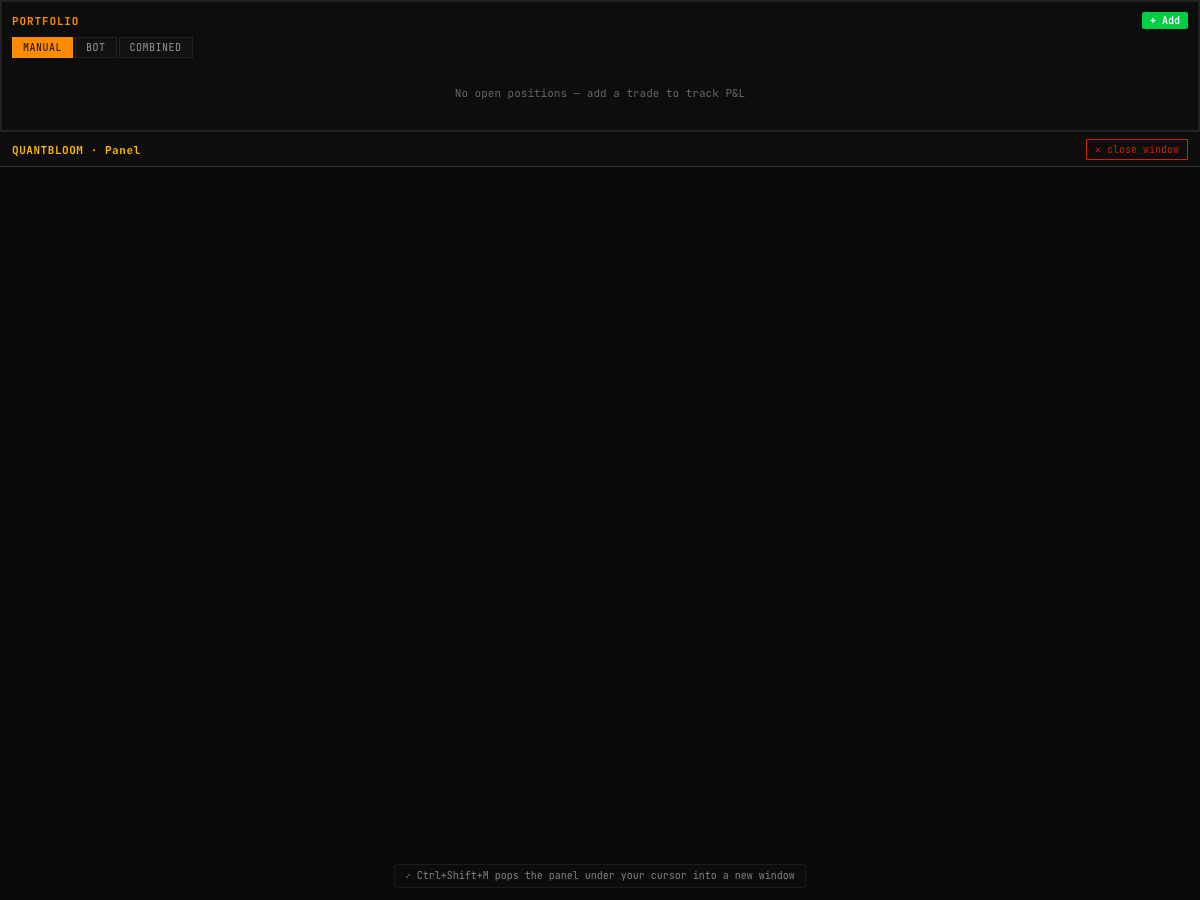
\includegraphics[keepaspectratio,alt={Portfolio}]{img/portfolio.png}}
\emph{Figure 15. Portfolio --- positions with live P\&L, weights, and
source tagging (manual vs.~bot).}

\pandocbounded{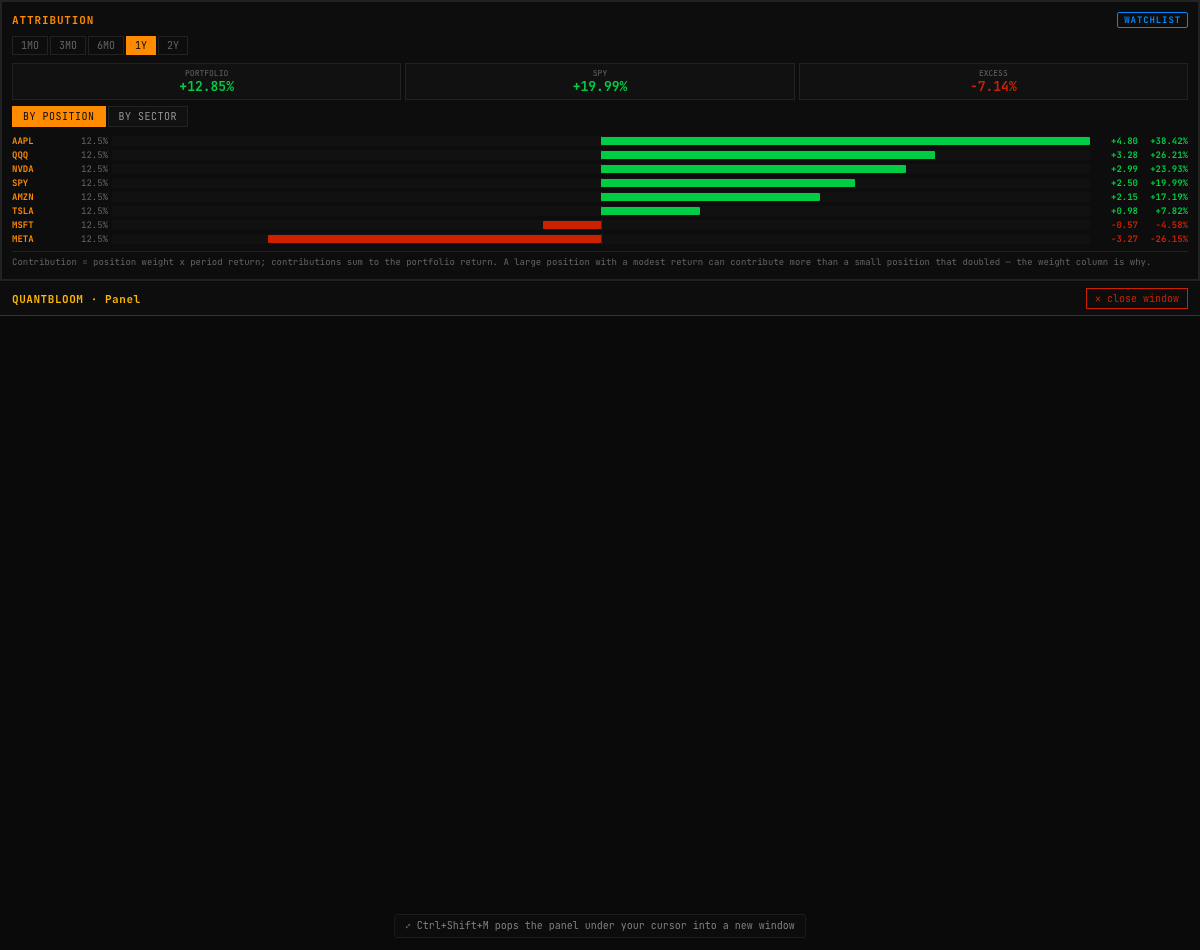
\includegraphics[keepaspectratio,alt={Attribution}]{img/attribution.png}}
\emph{Figure 16. Performance attribution --- return contribution by
position and sector against the benchmark.}

\pandocbounded{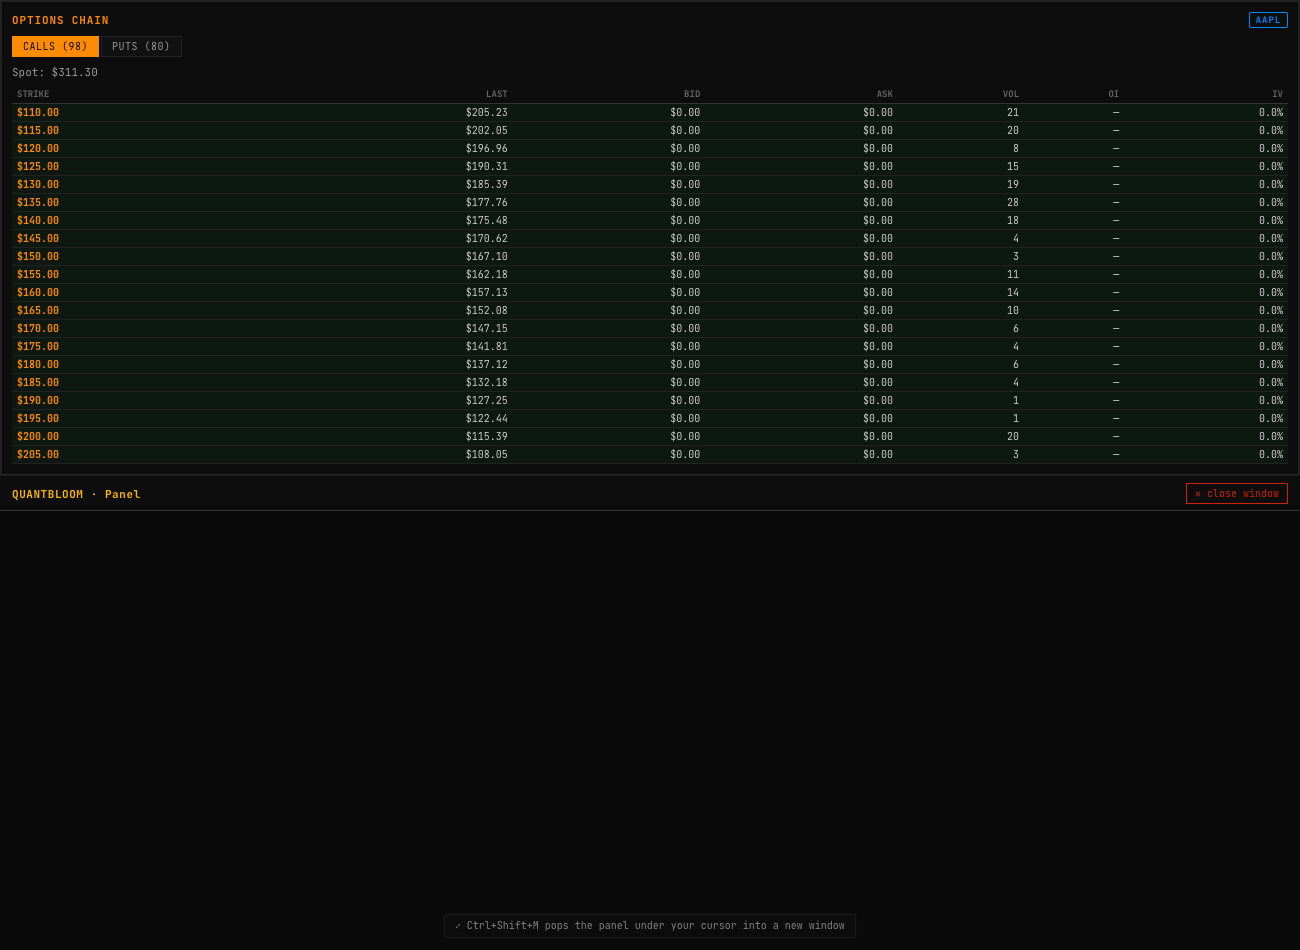
\includegraphics[keepaspectratio,alt={Options chain}]{img/options.png}}
\emph{Figure 17. The options chain with Black-Scholes Greeks (delta,
gamma, theta, vega) and numerically-solved implied volatility.}

\pandocbounded{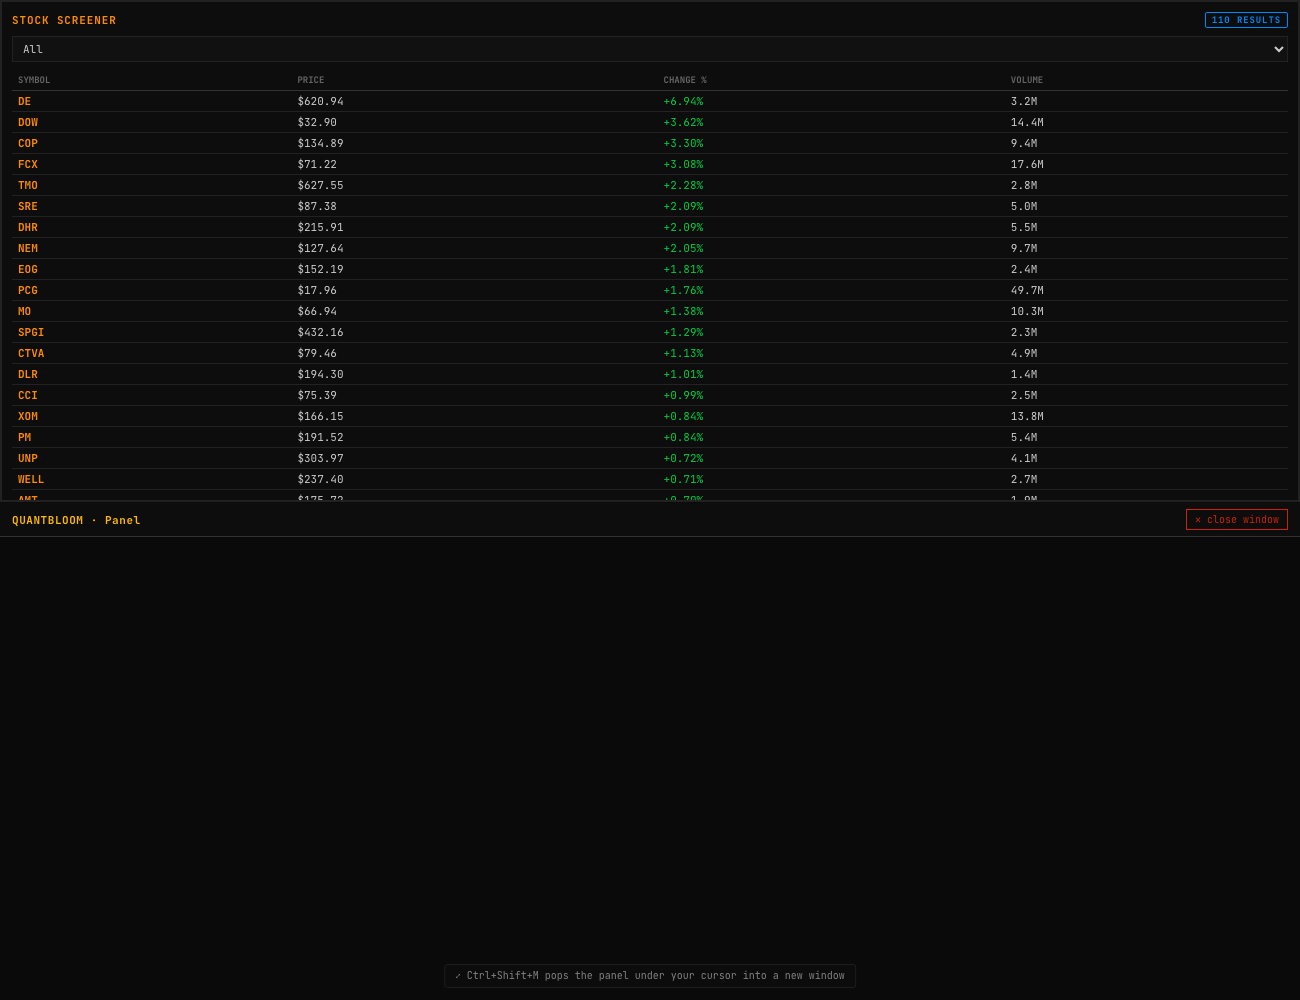
\includegraphics[keepaspectratio,alt={Stock screener}]{img/screener.png}}
\emph{Figure 18. The stock screener --- filtering the universe on
fundamental and technical criteria.}

\pandocbounded{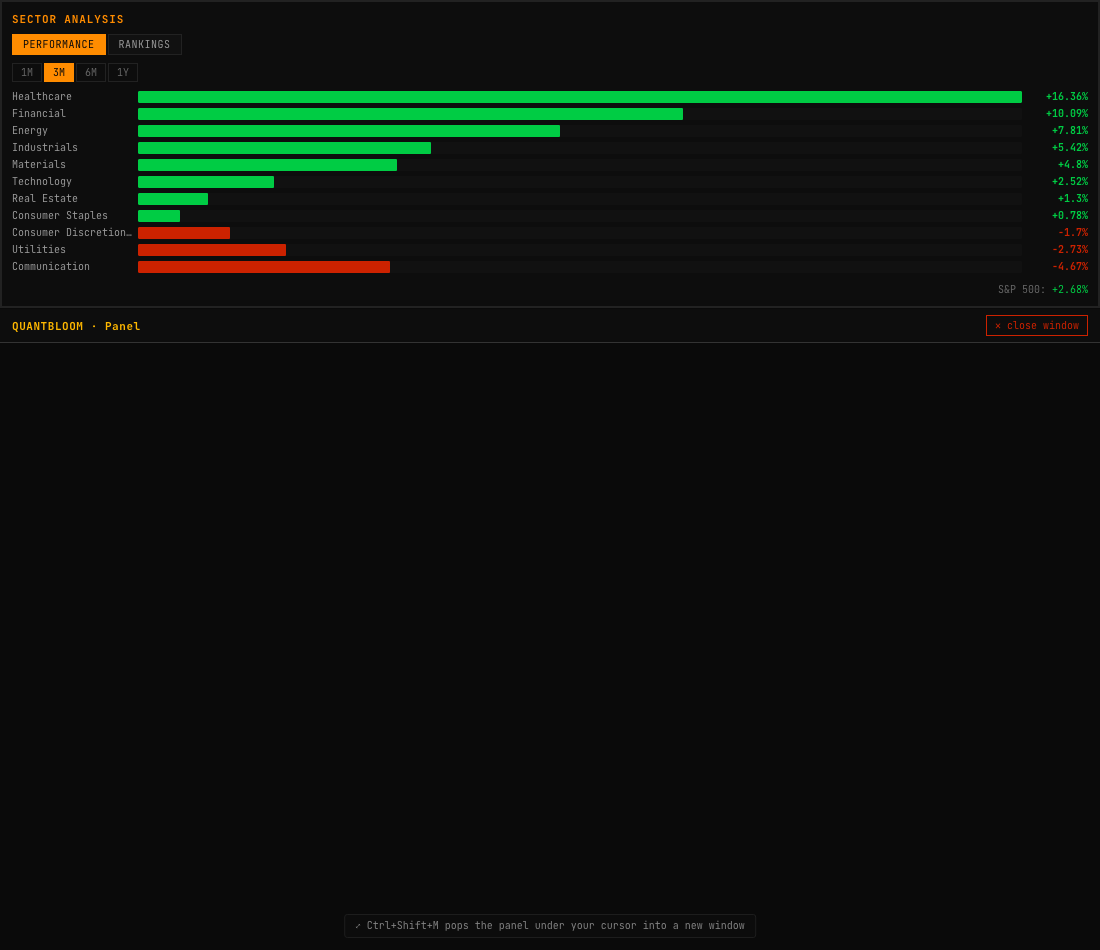
\includegraphics[keepaspectratio,alt={Sector analysis}]{img/sector.png}}
\emph{Figure 19. Sector analysis --- a heat-tiled view of relative
sector performance.}

\pandocbounded{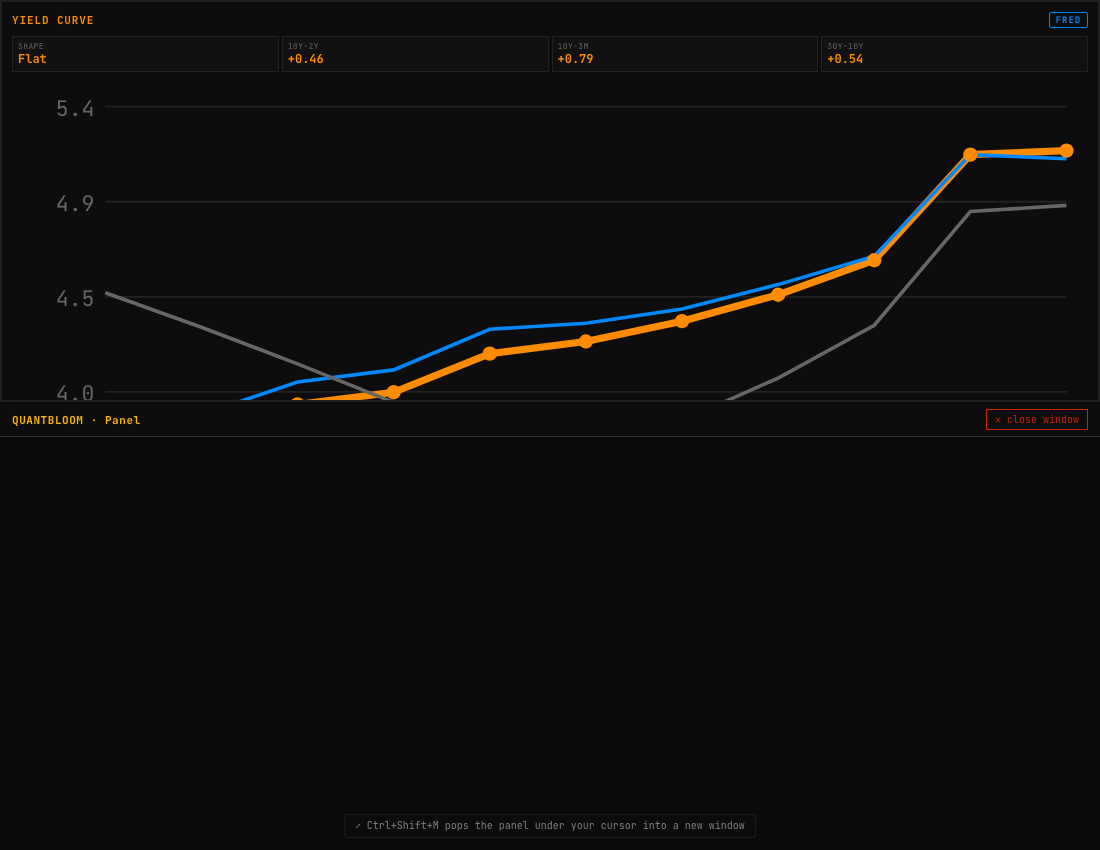
\includegraphics[keepaspectratio,alt={Yield curve}]{img/yield-curve.png}}
\emph{Figure 20. The Treasury yield curve from FRED, with key spreads.}

\pandocbounded{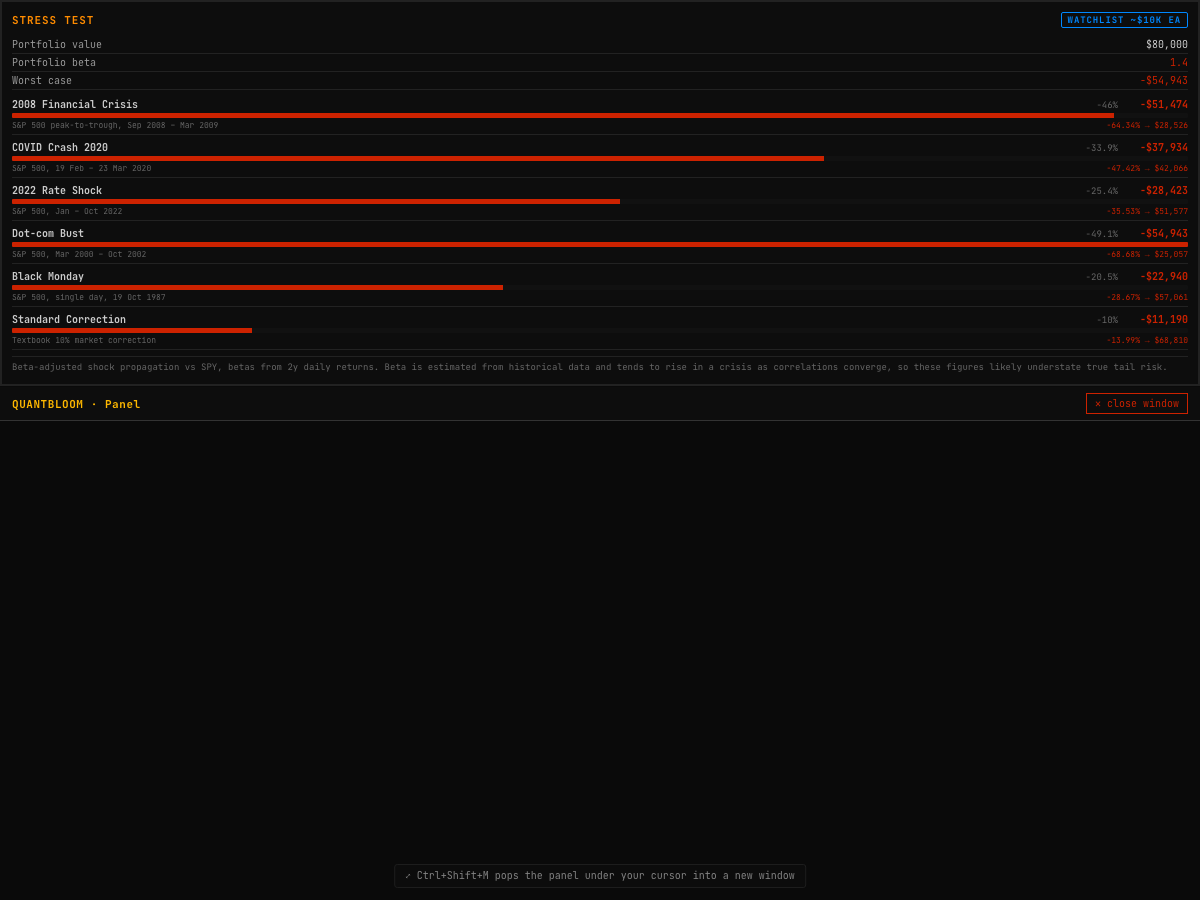
\includegraphics[keepaspectratio,alt={Stress test}]{img/stress-test.png}}
\emph{Figure 21. Stress testing --- replaying historical crises and
custom shocks against the current book via beta-adjusted propagation.}

\pandocbounded{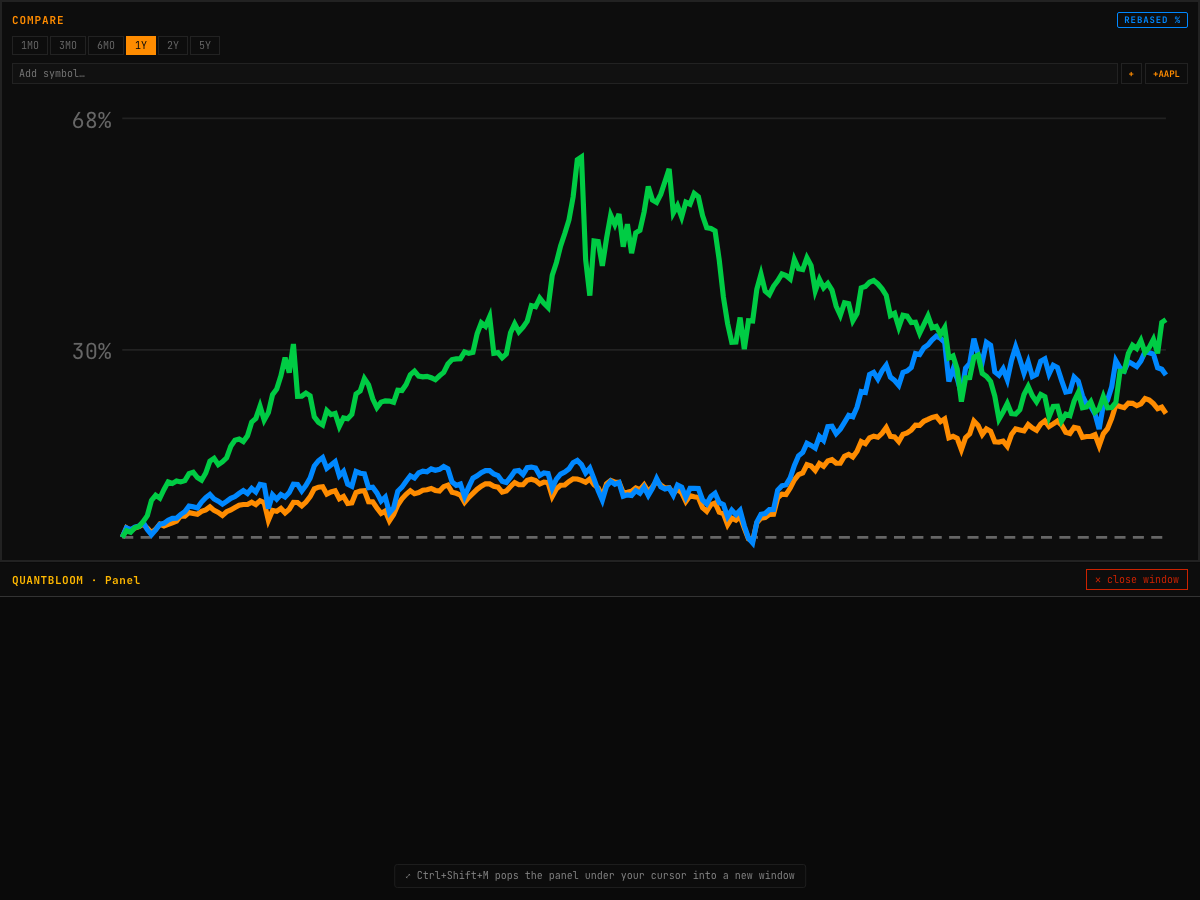
\includegraphics[keepaspectratio,alt={Cross-asset compare}]{img/compare.png}}
\emph{Figure 22. Rebased cross-asset comparison --- several instruments
normalised to a common base for relative-performance analysis.}

\subsubsection{References}\label{references}

\begin{enumerate}
\def\labelenumi{\arabic{enumi}.}
\tightlist
\item
  M. López de Prado, \emph{Advances in Financial Machine Learning},
  Wiley, 2018 (triple-barrier labelling; the Deflated Sharpe Ratio; CSCV
  / PBO).
\item
  D. Bailey and M. López de Prado, ``The Deflated Sharpe Ratio:
  Correcting for Selection Bias, Backtest Overfitting, and
  Non-Normality,'' \emph{Journal of Portfolio Management}, 2014.
\item
  J. H. Friedman, ``Greedy Function Approximation: A Gradient Boosting
  Machine,'' \emph{Annals of Statistics}, 2001.
\item
  H. Markowitz, ``Portfolio Selection,'' \emph{Journal of Finance},
  1952.
\item
  N. Somani, \emph{Power 2026: Electricity Pricing in the Age of AI}
  (merit-order pricing, LMP and transmission congestion, spark spreads,
  heat-rate call options, the duck curve, scarcity pricing).
\item
  F. Black and M. Scholes, ``The Pricing of Options and Corporate
  Liabilities,'' \emph{Journal of Political Economy}, 1973.
\end{enumerate}

\begin{center}\rule{0.5\linewidth}{0.5pt}\end{center}

\emph{QuantBloom Terminal is a research and education platform. Nothing
in this document is investment advice, and no metric is a prediction.
The trading bot targets a paper account by default; backtested
performance does not predict future returns.}

\end{document}
